% 来源: 19c9fb8c-1472-8ce1-8000-0000e6372a9d_1.2_网络算法学.pdf
% 提取时间: 2026-02-28T22:51:20+08:00

网络算法学
1.2 技术：网络算法学
在本书中，我们将讨论许多具体技术：中断、拷贝和时间轮；Pathfinder和Sting；为什么有些路由器非
常慢；Web服务器是否可以扩展。但是，贯穿本书并使它不仅仅是一本食谱的是网络算法学的概念。如
前所述，网络算法学认识到采用系统方法简化网络实现的重要性。
虽然每个人都知道互联网是由路由器和链路组成的系统，但可能不太明显的是，从Cisco GSR到Apache
Web服务器的每个网络设备也是一个系统。系统由在不同时间点实例化的互连子系统构成。例如，核心
路由器由带有转发引擎和数据包存储器的线路卡组成，这些线路卡通过交叉开关连接。路由器的行为受
到各个时间尺度决策的影响，这些时间尺度从制造时间（当默认参数存储在NVRAM中时）到路由计算时
间（当路由器协同计算路由时）再到数据包转发时间（当数据包被发送到相邻路由器时）。
因此，系统方法中的一个关键观察是，通常可以通过将某些功能在空间上（即移动到其他子系统）或时
间上（即在功能显然需要之前或之后的时间点）移动来设计高效的子系统。从某种意义上说，网络算法
学的实践者是一个不择手段的机会主义者，愿意随时改变规则以使游戏变得更容易。唯一的限制是整个
系统提供的功能继续满足用户的需求。
在马克·吐温的一本书中，一个康涅狄格州的美国佬被传送回亚瑟王的宫廷。然后，这位美国佬用枪与习
惯于用长矛决斗的骑士作战。这是改变系统假设（用枪代替长矛）来解决问题（赢得决斗）的一个例
子。
考虑到网络实现者在高速下所面临的限制——日益复杂的任务、支持更大的系统、少量高速内存和少量
的内存访问——可能需要动用武器库中的每一个技巧、每一把枪来跟上互联网不断增长的速度和规模。
设计者可以投入硬件、改变系统假设、设计新算法——无论采取什么措施都要完成任务。
本书分为四个部分。第一部分是本书的第一章，为将网络算法学应用于数据包处理奠定了基础。第一部
分的第二章概述了模型，第三章介绍了本书其余部分使用的一般原则。




\begin{figure}[htbp]
\centering
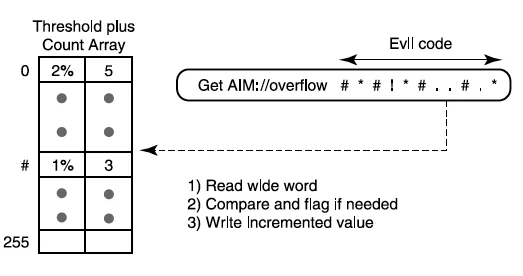
\includegraphics[width=0.8\textwidth]{../assets/ch01/ch01-1_2_网络算法学-003.png}
\end{figure}
图1.3 通过注意到非打印字符的频率来察觉恶意数据包。
快速了解网络算法学的一个好方法是立即进入一个热身示例。虽然下面的热身示例是在可以设计新硬件
的网络设备上下文中，但请注意，第二部分是关于仅使用软件设计技术构建高效服务器的。

                                                    1
1.2.1 热身示例：察觉恶意数据包
想象一下，在企业网络边缘的前端网络监视器（或入侵检测系统）希望标记可疑的传入数据包——可能
包含对内部计算机攻击的数据包。一种常见的此类攻击是缓冲区溢出攻击，攻击者在网络头部字段F中放
置机器代码C。
如果接收计算机为头部字段F分配的缓冲区太小，并且在检查溢出时疏忽大意，代码C可能会溢出到接收
机器的堆栈上。经过更多努力，入侵者可以让接收机器实际执行恶意代码C。然后C接管接收机器。图1.3
展示了这种攻击在一个熟悉的领域中的体现，即目标Web URL（统一资源定位符）。监视器如何检测到
这种可疑URL的存在呢？一种可能的方法是观察到包含恶意代码的URL通常过长（一个简单的检查），
并且通常包含大量不寻常（至少在URL中）的字符，如#。因此，监视器可以将这些数据包（包含过长且
包含过多此类不寻常字符的URL的数据包）标记出来进行更彻底的检查。
值得在一开始就说明，这种策略的安全影响需要仔细考虑。例如，可能有一些无害的程序，如CGI脚本，
在URL中导致误报。在不深入探讨整体架构影响的情况下，让我们假设这是安全架构师交给芯片架构师
的一个规范。我们现在使用这个由Mike Fisk提出的示例问题来说明算法学的实际应用。
面对这样的规范，芯片设计师可能会使用以下设计过程，该过程说明了一些网络算法学的原则。该过程
从一个初步设计方案开始，并使用更好的算法、放宽规范和利用硬件等技术对设计进行改进。
1.2.2 初步方案
检查整体长度很容易实现，因此我们专注于检查可疑字符的普遍性。第一个初步方案如\begin{figure}[htbp]
\centering
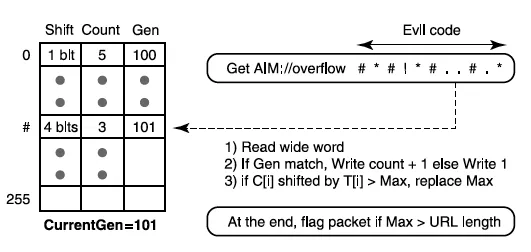
\includegraphics[width=0.8\textwidth]{../assets/ch01/ch01-1_2_网络算法学-004.png}
\end{figure}
图1.4所示。芯片
维护两个数组T和C，每个数组有256个元素，对应8位字符的每个可能值。阈值数组T包含每个字符的可
接受百分比（作为整个URL长度的一部分）。如果URL中某个字符的出现次数超过这个百分比，就应该
标记该数据包。每个字符可以有不同的阈值。
计数数组C中间部分，包含每个可能字符i的当前计数C[i]。当芯片读取URL中的新字符“i”时，它将C[i]增
加1。对于所有i的值，C[i]在遇到新数据包时初始化为0。计数过程在芯片解析HTTP头部并识别URL开始
                                                     2
后启动。
在HTTP中，URL的结束由两个换行符表示；因此，只有在解析完整个URL字符串后才能知道URL的长
度。因此，在URL结束后，芯片对数组C进行最终遍历。如果对于任何j，C[j]≥L·T[j]，其中L是URL的长
度，则标记该数据包。
假设数据包以高速进入监视器，并且我们希望在下一个数据包到达之前完成对一个数据包的处理。这种
要求称为线速处理，在网络中非常常见；它即使在最坏情况下也能防止处理积压。为了满足线速要求，
理想情况下芯片应该对每个URL字节执行少量恒定数量的操作。假设递增计数器的主要步骤可以在接收
一个字节的时间完成。
不幸的是，首先遍历数组初始化它，然后遍历数组检查阈值违规，这使得这个设计速度变慢。最小数据
包大小通常只有40个字节，并且只包含网络头部。再加上768次更多操作（对C的每个元素进行1次写入
和1次读取，并对256个索引中的每一个读取T），这可能使得这个设计不可行。
1.2.3 算法思维
直观上，第二遍遍历数组C和T似乎是浪费。例如，如果任何字符超过阈值就足够报警了。那么为什么要
检查所有字符呢？这表明只需要跟踪到目前为止遇到的最大字符计数c；也许算法只需要检查c是否相对
于总URL长度L超过阈值。




\begin{figure}[htbp]
\centering
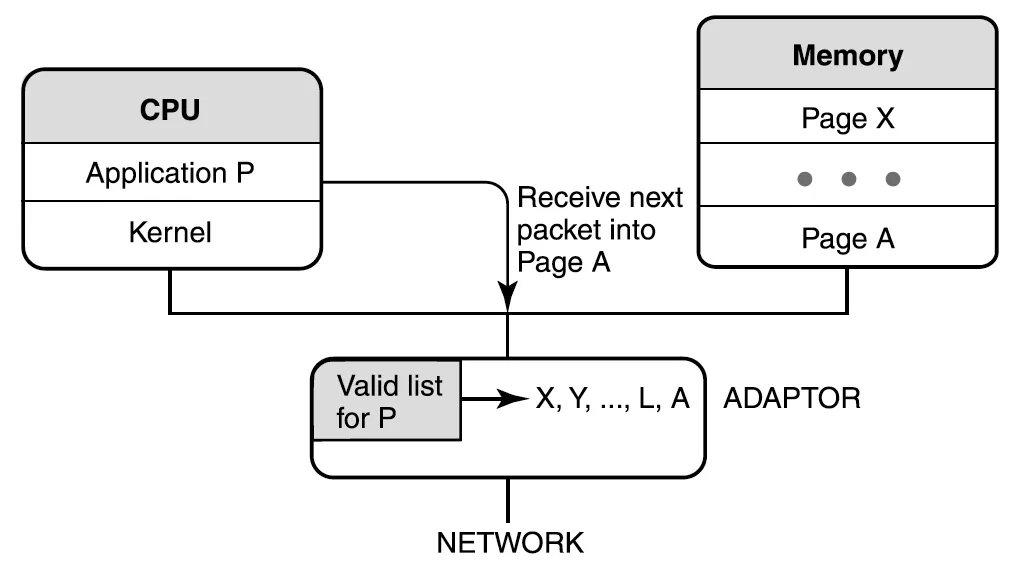
\includegraphics[width=0.8\textwidth]{../assets/ch01/ch01-1_2_网络算法学-005.png}
\end{figure}
图1.5
通过跟踪最高相对计数值Max来避免最后循环遍历阈值数组，该值对应于迄今为止遇到的某个字符k，使
得C[k]/T[k]=Max是所有遇到字符中最高的。如果读取到一个新字符i，芯片增加C[i]。如果
C[i]/T[i]>Max，则芯片用C[i]/T[i]替换当前存储的Max值。在URL处理结束时，如果Max≥L，芯片发出
警报。
这是为什么有效的。如果Max=C[k]/T[k]≥L，显然必须标记该数据包，因为字符k超过阈值。另一方面，
如果C[k]/T[k]<L，那么对于任何字符i，都有C[i]/T[i]≤C[k]/T[k]<L。因此，如果Max低于阈值，则没有
字符超过阈值。因此不可能出现漏报。这个解决方案如图1.5所示。
                                                               3
1.2.4 改进算法：利用硬件
新算法消除了最后的循环，但仍然需要在处理每个字节时进行除法运算。除法逻辑相当复杂，如果可能
的话应该避免——但如何避免呢？
回到规范及其预期用途，看起来阈值不太可能是精确的浮点数。提供阈值的架构师不太可能精确估计这
些值；将2.78%近似为3%而不显著影响安全目标是可能的。那么为什么不进一步将阈值近似为小于精确
目标阈值的2的幂次方呢？因此，如果阈值是1/29，为什么不将其近似为1/32？
以这种方式改变规范需要与系统架构师协商。假设架构师同意这个新提议。那么阈值如1/32可以紧凑地
编码为相应的2的幂次方——即5。这个阈值移位值可以存储在阈值数组中，而不是分数。
因此，当遇到字符j时，芯片像往常一样增加C[j]，然后根据指定的阈值将C[j]左移——除以1/x等同于乘
以x。如果移位后的值高于Max的最后存储值，则芯片用新值替换旧值并继续处理。
因此，处理一个字节所需的逻辑是一个简单的移位和比较。存储状态只是一个寄存器来存储Max。目
前，该设计需要读取阈值数组（读取移位值）、读取计数数组（读取旧计数值）和写入计数数组（写回
增加后的值）。
现在，内存访问——即使是对于最快的片上内存也需要1-2纳秒，对于较慢的内存可能需要长达10纳秒
——比逻辑慢。单个门延迟只有皮秒级，移位逻辑不需要太多门延迟。因此，处理瓶颈在于内存访问次
数。
芯片实现可以通过将两次内存读取合并为一次来优化，如\begin{figure}[htbp]
\centering
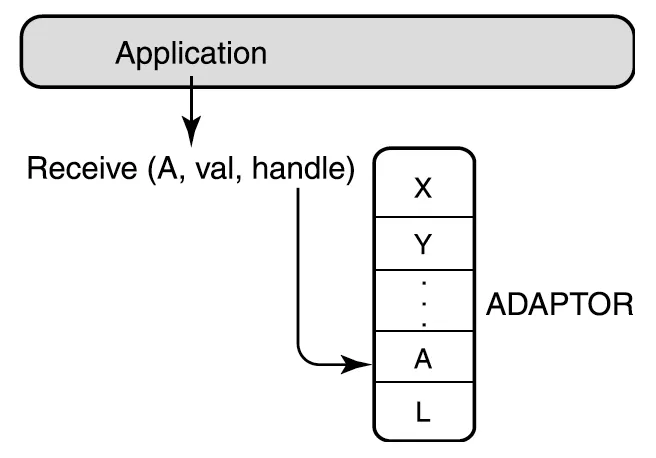
\includegraphics[width=0.8\textwidth]{../assets/ch01/ch01-1_2_网络算法学-006.png}
\end{figure}
图1.6所示。思路是将计数数组和阈值数组合并
为一个更宽的数组。具体来说，使内存字足够宽以容纳计数器（例如，15位来处理长度为32K的数据
包）和阈值（根据所需精度，最多14位）。这样两个字段可以轻松合并成一个更大的字，大小为29位。
实际上，硬件可以处理远大于此的字长，高达1000位。此外，请注意，在软件中提取打包在单个字中的
两个字段相当繁琐，而在硬件中通过适当路由寄存器之间的连线或使用多路复用器则轻而易举。




图1.6

                                                   4
通过合并计数和阈值数组，将两次读取合并为一次，利用宽字和合并数组。
1.2.5 清理工作
我们一直推迟讨论一个棘手的问题。终端循环已经消除，但初始初始化循环仍然存在。要处理这个问
题，请注意芯片在解析完当前数据包的URL后、遇到下一个数据包的URL前有空闲时间。
不幸的是，即使有HTTP头部，数据包也可能小至50字节。因此，即使假设除了URL的10个字节外还有
40个非URL字节的空闲时间，这仍然不足以在无需每字节额外支付6次操作的情况下初始化一个256字节
的数组——每次URL处理过程中每个数组元素需要一次读取和一次写入。
像懒人一样，一种策略是将工作推迟到绝对必要时再进行，希望它可能永远不需要。请注意，严格来
说，芯片不需要在当前数据包中第一次访问字符i之前初始化C[i]。但是芯片如何知道它是第一次看到字
符i呢？
为了实现惰性求值，每个表示合并数组中条目的内存字必须扩展，比如增加一个3位代号G[i]。代号可以
看作是以数据包为单位测量的时钟时间，但它限制为3位。因此，除了每个i的额外G[i]外，芯片还维护另
一个寄存器g，也是3位长；g每处理一个数据包就递增模8。此外，每次更新C[i]时，芯片也会更新G[i]以
反映当前的g值。
有了代号，芯片就不需要在当前数据包处理完后初始化计数数组了。然而，考虑一个代号为h的数据包，
其中包含URL中的字符i。当芯片在处理该数据包时遇到i时，芯片从计数数组中读取C[i]和G[i]。如果
G[i]≠h，这清楚地表明条目i上次被较早的数据包访问过且之后未初始化。因此，逻辑会将C[i]的值写回
为1（初始化加递增）并将G[i]设置为h。如\begin{figure}[htbp]
\centering
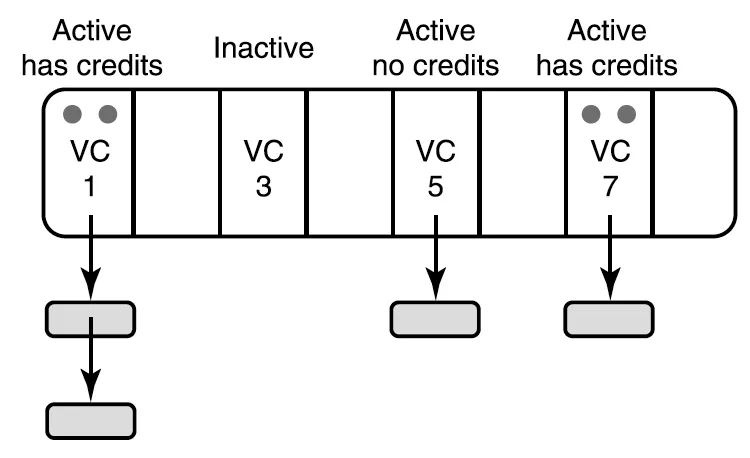
\includegraphics[width=0.8\textwidth]{../assets/ch01/ch01-1_2_网络算法学-007.png}
\end{figure}
图1.7所示。




图1.7
最终解决方案通过代号巧妙地处理初始化循环。
细心的读者会立即提出异议。由于代号只有3位，一旦g的值回绕，就会出现别名问题。因此，如果G[i]为
5且条目i直到八个数据包后才被访问，g将回绕到5。如果下一个数据包包含i，C[i]将不会被初始化，计

                                                   5
数将（错误地）累积当前数据包中的i的计数以及八数据包之前的计数。
芯片可以通过执行一个单独的"清理"循环来解决这种别名问题，该循环读取数组并将所有带有过期代号的
计数器初始化为0。为了正确性，芯片必须保证每处理八个数据包就对数组进行一次完整扫描。假设每个
数据包有（比如说）40个非URL字节空闲时间，这保证了在处理八个数据包后有320个非URL字节的空
闲时间，足以使用每次读取和写入一个字节的方式初始化一个256元素数组，无论该字节是URL字节还是
非URL字节。显然，如果需要更多空闲时间，设计者可以通过增加代号的位数来获得更多空闲时间，代
价是数组中稍微增加的存储空间。
因此，芯片必须有两种状态：一种用于处理URL字节，另一种用于处理非URL字节。当URL完全处理完
后，芯片切换到"清理"状态。芯片维护另一个寄存器，指向要清理的下一个数组条目s。在清理状态下，
当接收到非URL字符时，芯片读取合并数组中的条目s。如果G[s]≠g，则将G[s]重置为g并将C[s]初始化
为0。
因此，使用每个数组条目额外的3位代号减少了初始化处理周期，通过用存储换取处理。总的来说，现在
一个合并数组条目只有32位，15位用于计数器，14位用于阈值移位值，3位用于代号。请注意，在URL字
节处理期间所需的额外初始化检查并没有增加内存引用（瓶颈），但略微增加了处理逻辑。此外，它需
要两个额外的芯片寄存器来保存g和s，这是一笔很小的额外开销。
1.2.6 网络算法学的特点
检测恶意数据包的示例说明了网络算法学的三个重要方面：
a. 网络算法学是跨学科的：鉴于网络处理必须以高速完成，路由器设计者很难不使用硬件。该示例利用
了硬件的几个特性：它假设可以轻松实现任意大小的宽字；它假设移位比除法更容易；它假设内存引用
是瓶颈；它假设片上快速内存中包含256元素数组是可行的；它假设增加几个额外寄存器是可行的；最后
它假设对逻辑进行小改动以结合URL处理和初始化是微不足道的。
对于不熟悉硬件设计的读者来说，这有点像不懂数牌规则就加入一场纸牌游戏，然后发现自己以意想不
到的方式被出牌和压制。本书的一个论点是，掌握一些相关硬件设计知识可以帮助即使是软件设计师也
至少理解不同硬件设计的可行性。本书的另一个论点是，这种跨学科思维有助于产生最佳设计。
因此，第2章介绍了游戏规则。它介绍了硬件、操作系统和网络的简单模型，指出了解决棘手实现问题的
机会。它还介绍了操作系统和网络的简单模型。之所以这样做，是因为像客户端和Web服务器这样的终
端系统需要调整和理解操作系统问题以提高性能，就像路由器和网络设备需要调整硬件一样。
b. 网络算法学认识到系统思维的首要性：规范被放宽以允许近似阈值为2的幂次方，这简化了硬件。放宽
规范和将工作从一个子系统转移到另一个子系统是一种极其常见的系统技术，但这并不是当前大学教育
实践中鼓励的做法，在大学教育中，每个领域都是孤立教授的。
因此，今天有独立的算法课程、操作系统课程和网络课程。这往往鼓励"黑箱"思维，而不是整体或系统思
维。该示例还提到了其他系统技术，如使用惰性求值和用存储换取处理来清理计数数组。
                                                     6
因此，本书的一个特点是试图将算法学中使用的系统原则提炼为15条原则，这些原则列在书的前封面
上，并在第3章中详细探讨。本书试图用这些原则来解释和剖析本书中描述的所有网络实现。这些原则也
标有编号以便于参考，尽管在大多数情况下，我们会同时使用编号和名称。例如，快速浏览前封面你会
发现放宽规范是原则P3，惰性求值是P2b。
c. 网络算法学可以从算法思维中受益：虽然本书强调系统思维的首要性以尽可能巧妙地解决问题，但在
许多情况下系统约束阻止了问题的完全消除。在我们的示例中，在尝试通过放宽规范来巧妙解决问题
后，误报问题导致考虑跟踪相对于其阈值最高的计数器。作为第二个例子，第11章表明，尽管尝试使用所
谓的标签交换来巧妙解决互联网查找问题，许多路由器仍然采用高效算法进行查找。
然而，值得强调的是，由于模型与标准理论模型有所不同，仅仅盲目重用现有算法往往是不够的。例
如，第13章讨论了需要在8纳秒内调度交叉开关的需求，这导致考虑更简单的最大匹配启发式算法，而不
是产生二分图中最优匹配的更复杂算法。
作为第二个例子，第11章描述了BSD实现如何盲目重用一种称为Patricia trie的数据结构来进行IP查找，
该数据结构使用跳过计数，导致算法需要复杂的回溯。一种简单的修改保留了实际跳过的位（而不是计
数），避免了回溯的需要。但这需要对黑盒（即算法）及其应用有一定的洞察力。
总之，不加批判地使用标准算法可能会因为不恰当的度量（例如，对于像BPF这样的数据包过滤器，插
入新分类器可能比搜索需要更多时间）、不恰当的模型（例如，忽略软件中的缓存行或硬件中的并行性
的影响）和不恰当的分析（例如，隐藏了确保线速转发的关键常数因子的大O复杂度结果）而错过实现突
破。
因此，本书的另一个目的是说服实现者，掌握算法洞察力和使用基本算法技术（如分治法和随机化）对
于设计高速网络处理任务至关重要。这引出了以下定义：
定义：网络算法学是采用跨学科系统方法，并辅以算法思维，在服务器、路由器和其它网络设备上设计
高速网络处理任务实现的技术。
本书的第一部分致力于更详细地描述网络算法学方法。第1章的前言部分给出了概述。
 重点            动机           示例主题
 模型            理解操作系统、硬件、网 内存技术技巧（交错、混合
               络的简单模型       SRAM/DRAM）
 策略            学习克服瓶颈的系统原则 传递提示、惰性评估、增加状态、利用
                            局部性
 问题            练习将原则应用于简单问 为网络监视器设计查找引擎
               题
\begin{figure}[htbp]
\centering
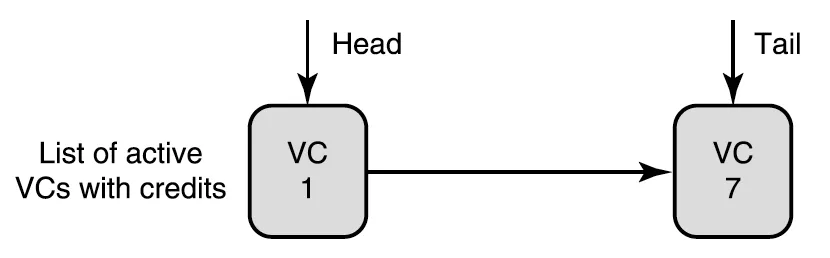
\includegraphics[width=0.8\textwidth]{../assets/ch01/ch01-1_2_网络算法学-008.png}
\end{figure}
图1.8

                                                       7
网络算法学预览。网络算法学通过一组模型、策略和示例问题引入，这些内容在第1章中描述。
虽然本书侧重于网络，但通用算法学方法适用于任何计算机系统的实现，无论是数据库、处理器架构还
是软件应用。第3章通过提供计算机系统实现领域的示例来提及这一更广泛的哲学。只对网络感兴趣的读
者可以放心，除了第3章外，本书其余部分避免了超出网络范围的进一步离题。
虽然第2部分和第3部分为重要特定问题提供了具体技术，但本书的主要目标是使读者能够在软件或硬件
中高速处理任意数据包处理任务。因此，未来的实现者可能会被赋予加速Web服务器中的XML处理（鉴
于当前趋势很可能）甚至在路由器中计算卡方统计量（因为卡方提供了一种检测入侵检测等任务中观察
到的异常频率的测试）的任务。尽管被分配了一个完全陌生的任务，希望实现者能够使用本书描述的模
型、原则和技术来设计这些任务的新解决方案。
十五个实施原则
与其计算，我不得不思考问题，这是一种成功的公式，我强烈推荐。
——伊万·苏泽兰
在理解了国际象棋游戏中皇后和骑士的移动方式之后，了解基本策略（如在残局中将兵升变和王车易
位）是有帮助的。同样，在上一章学习了协议实现游戏的一些规则之后，本章将以15个原则的形式向您
介绍实施策略。这些原则是从运行良好的协议实现中抽象出来的。许多优秀的实现者无意识地使用这些
原则。然而，关键是要阐明这些原则，以便可以有意识地应用它们来制定高效的实现。
本章的结构如下。3.1节通过一个三值内容可寻址存储器（CAM）问题来激励使用这些原则。3.2节使用
网络安全取证问题来澄清算法和算法学之间的区别。3.3节介绍了15个实施原则；3.4节解释了实施原则
和设计原则之间的区别。最后，3.5节描述了在应用这些原则之前应提出的一些警示性问题。
快速参考指南
时间紧迫的读者应查阅\begin{figure}[htbp]
\centering
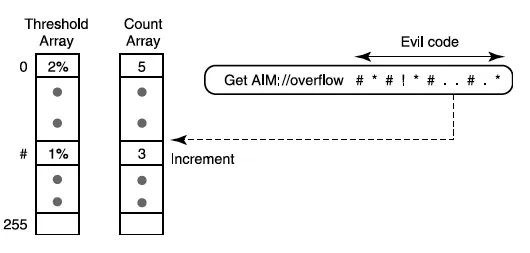
\includegraphics[width=0.8\textwidth]{../assets/ch01/ch01-1_2_网络算法学-001.png}
\end{figure}
图3.1-3.3中总结的15个原则。这些原则的两个网络应用可以在三值CAM更新问题
（第3.1节）和网络安全取证问题（第3.2节）中找到。
3.1 激励使用原则——更新三值内容可寻址存储器
如果一个字符串包含的字符是0、1或*，其中表示可以匹配0和1的通配符，则称该字符串为三值字符串。
长度为3的三值字符串示例包括S1=01和S2=1；实际的二进制字符串011同时匹配S1和S2，而111仅匹配
S2。三值内容可寻址存储器（CAM）是一种包含指定长度的三值字符串及其相关信息的内存；当输入一
个字符串时，CAM会并行搜索其所有内存位置，并在一个周期内输出匹配指定输入键的最低内存位置。
 编号               原则                 应用

                                                     8
P1                避免明显的浪费           零拷贝接口
P2 P2a P2b P2c    在时间上转移计算 预先计算 懒   应用设备通道 写时复制 集成层
                  惰求值 共享费用，批量处理     处理
P3 P3a P3b P3c    放宽系统要求 用时间换取确定    随机公平排队 交换机负载均衡
                  性 用时间换取准确性 在空间上   IPv6分片
                  转移计算
P4 P4a P4b P4c    利用系统组件 利用局部性 用速   基于局部性的接收器处理；
                  度换取内存 利用现有硬件      Lulea IP查找 快速TCP校验和
P5 P5a P5b P5c    添加硬件 使用内存交错和流水    流水线IP查找 共享内存交换机
                  线 使用宽字并行性 有效结合    维护计数器
                  DRAM和SRAM

图3.1
原则1-5的总结——系统思维。
 编号               原则                网络示例
 P6               创建高效的专业化例程        UDP校验和
 P7               避免不必要的通用性         Fbufs
 P8               不要拘泥于参考实现         回调
 P9               在层接口中传递提示         数据包过滤器
 P10              在协议头中传递提示         标签交换

\begin{figure}[htbp]
\centering
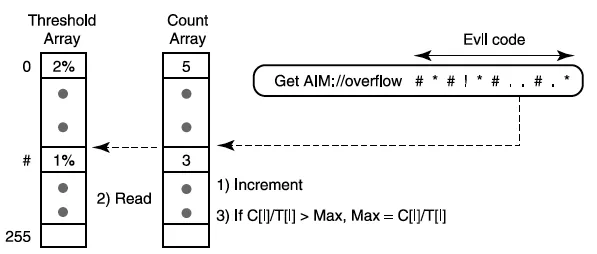
\includegraphics[width=0.8\textwidth]{../assets/ch01/ch01-1_2_网络算法学-002.png}
\end{figure}
图3.2
原则6-10的总结——在保持模块化的同时恢复效率。
图3.4展示了三值CAM在互联网路由器的最长匹配前缀问题中的应用。对于每个传入的数据包，每个互联
网路由器必须从传入的数据包中提取一个32位的目标IP地址，并将其与转发数据库中的IP前缀及其对应
的下一跳进行匹配。IP前缀是一个长度为32的三值字符串，其中所有的通配符都在末尾。我们将稍微改
变符号表示法，让表示任意数量的通配符字符，因此101匹配10100而不仅仅是1010。

                                                          9
编号                原则                网络示例
P11 P11a          优化期望情况 使用缓存       头部预测 Fbufs
P12 P12a          增加状态以提高速度 增量计算    活动VC列表 重新计算CRC
P13               优化自由度             IP前缀树查找
P14               使用桶排序、位图          定时轮
P15               创建高效的数据结构         第4层交换

图3.3
原则11-15的总结——加速关键例程。
图3.4
使用三值CAM进行前缀查找的示例。
因此，在图3.4中，发送到以010001开头的目标地址的数据包匹配前缀010001和01，但应根据互联网转
发的最长匹配规则发送到端口P5。我们将在第11章中详细讨论这个问题。现在，请注意，如果前缀按图
3.4中的方式排列，使得所有较长的前缀都出现在较短前缀之前（如图3.4所示），三值CAM可以在一个
内存周期内提供匹配的下一跳。
虽然三值CAM在消息转发方面非常快速，但它们要求较长的前缀必须出现在较短的前缀之前。然而，路
由协议经常添加或删除前缀。假设在图3.4中，必须向路由器数据库中添加一个新前缀11*，下一跳为端口
1。插入的朴素方法将通过在长度为2的前缀组中创建一个空位（即在0*之前创建一个空位）来实现，方
法是将所有长度为2或更长的前缀向上移动一位。
不幸的是，对于一个典型核心路由器所维护的大约100,000个前缀的大型数据库，这将需要100,000个内
存周期，这将使得添加前缀变得非常缓慢。我们可以通过系统地应用以下两个原则（在本章后面描述为
原则P13和P15）来获得更好的解决方案。
理解和利用自由度
观察图3.4中的转发表，我们看到所有相同长度的前缀都排列在一起，并且所有长度为i的前缀都出现在长
度为j>i的前缀之后。然而，在图中，所有相同长度的前缀也按值排序。因此，00出现在01之前，01出现
在10之前。但对于CAM来说，正确返回最长匹配前缀并不是必需的：我们只需要在不同长度的前缀之间
进行排序；我们不需要对相同长度的前缀进行排序。

                                                     10
观察图3.4的更抽象视图（如图3.5所示），我们看到，如果我们要在长度为i的前缀集合的开头添加一个
条目，我们必须在长度为i+1的前缀集合的末尾创建一个空位。因此，我们必须将已经位于此位置的条目
X移动到另一个位置。如果我们把X向上移动一步，我们将被迫回到之前低效的解决方案。
然而，我们对自由度的观察表明，我们可以将X放置在任何靠近其他长度为i+1前缀的位置。因此，另一
种想法是将X移动到Y的位置，Y是最后一个长度为i+2的前缀。但这又迫使我们为Y找到一个新位置。这
如何帮助我们？我们需要第二个原则。
使用算法技术
递归再次被提出：我们通过将问题简化为同一问题的“更小”实例来解决问题。在这种情况下，为Y分配新
位置的问题的“更小”是因为长度为i+2的前缀集合比长度为i+1的前缀集合更接近CAM顶部的空位。因
此，我们从CAM的顶部开始向下工作，通过在长度为1的前缀集合的末尾创建一个空位，然后在长度为2
的前缀集合的末尾创建一个空位，依此类推，直到我们在长度为i的前缀集合的末尾创建一个空位。因
此，最坏情况下的时间复杂度是32-i次内存访问，对于小的i来说大约是32次。
我们完成了吗？没有，我们可以做得更好，通过进一步利用自由度。首先，在图3.5中，我们假设空位在
CAM的顶部。但空位可以放在任何地方。特别是，它可以放在长度为16前缀之后。这将最坏情况下的内
存访问次数减少了一半（Shah和Gupta，2001）。
一个更复杂的自由度是如下。到目前为止，CAM插入算法的规范要求“如果i>j，则长度为i的前缀必须出
现在长度为j的前缀之前。”这样的规范对于正确性来说是足够的，但并不是必需的。例如，010可以出现
在111001之前，因为没有地址可以同时匹配这两个前缀！
因此，一个不那么严格的要求是“如果两个前缀P和Q可以匹配同一个地址，那么如果P比Q长，则P必须
在CAM中出现在Q之前。”这在Shah和Gupta（2001）中被用来进一步减少某些实际数据库中插入的最
坏情况下的内存访问次数。
虽然最后的改进并不值得其复杂性，但它指向了另一个重要的原则。我们经常将一个大问题分解为子问
题，并将子问题交给基于规范的解决方案。例如，CAM硬件设计者可能已经将更新问题交给微码编写
者，指定较长的前缀必须放在较短的前缀之前。
但是，正如之前所述，这样的规范可能不是解决原始问题的唯一方法。因此，对规范进行更改（原则
P3）可以产生更高效的解决方案。当然，这需要有好奇心和自信的个体，他们能够理解全局，或者有足
够的勇气提出危险的问题。
3.2 算法与算法学
可能会有人争辩说，前面的例子本质上仍然是算法性的，并不需要系统思维。另一个快速的例子将有助
于澄清算法和算法学之间的区别。

                                                   11
安全取证问题
在许多入侵检测系统中，当某个源（例如，通过某些数据包头部定义的源IP地址）被判定为可能行为不
端时，管理员通常会发现该流（例如，发送了100,000个数据包到被攻击子网中的不同机器）的证据通常
已经消失（即，已经被路由器转发）。问题是，概率检查需要在一段时间内累积每个接收到的数据包的
某些状态（例如，在怀疑表中），以便在某个源被判定为可疑之前。因此，如果在10秒后被判定为可
疑，如何回溯并检索该源在这10秒内发送的数据包？
图3.6
保持一个包含过去可疑流发送的最后一个100,000个数据包的队列，其中包含关于可疑流的信息。
为了实现这一点，在图3.6中，我们保持一个由路由器发送的最后一个100,000个数据包的队列。当一个
数据包被转发时，我们还将该数据包的副本（或仅保留指向该数据包的指针）添加到队列的头部。为了
保持队列的有界性，当队列满时，我们从尾部删除数据包。
这种方案的主要困难在于，当一个可疑流被检测到时，队列中可能有很多该流的包（见图3.6）。所有这
些包都必须放入取证日志中以传输给管理员。教科书式的算法方法是为每个流ID添加一些索引结构，以
便快速搜索流ID。例如，可以维护一个流ID的哈希表，将每个流映射到队列中具有该流ID的所有数据包的
指针列表。当一个新的数据包放入队列时，在哈希表中查找流ID，并将新数据包在队列中的地址放在流
的列表末尾。当然，当数据包离开队列时，必须从列表中删除其条目，并且可以保证要删除的条目是该
流ID的第一个条目。
尽管如此，教科书式的方案仍然存在一些困难。它增加了维护每个流ID的额外队列的空间，并且在高速
实现中空间可能非常宝贵。它还增加了数据包处理的额外复杂性，以维护哈希表，并且需要在数据包被
100,000个数据包之后的数据包覆盖之前将流的所有数据包读出到取证日志中。相反，以下“系统”解决方
案可能更为优雅。
解决方案
当F被判定为可疑时，不要试图立即识别所有属于流F的数据包，而是在数据包到达队列末尾时懒惰地识
别它们。如图3.7所示，当我们将一个数据包添加到队列头部时，我们必须从队列尾部删除一个数据包
（至少当队列满时）。
保持一个包含过去可疑流发送的最后一个100,000个数据包的队列，其中包含关于可疑流的信息。
如果该数据包（例如，Q，见图3.6）属于流F，并且流F已达到某种怀疑阈值，我们然后将数据包Q添加
到取证日志中。日志可以发送给管理员。这种方案的额外开销很大，但可以管理；我们必须执行两个数
据包处理步骤，一个用于正在转发的数据包，另一个用于从队列中移除的数据包。但这两种数据包处理


                                                12
步骤在教科书式方案中也是必需的；另一方面，优雅的方案不需要哈希，并且使用的存储空间更少（不
需要在100,000个数据包之间建立指针）。
3.3 十五个实施原则——分类和描述
前面两个例子以及第1章中的热身练习激发了以下15个原则，这些原则将在本书的其余部分中使用。它们
在封面内侧进行了总结。为了增加结构，它们被分类如下：
 ● 系统原则：原则1-5利用了我们正在构建系统的事实。
 ● 在保持模块化的同时提高效率：原则6-10提出了一些方法，可以在允许复杂系统模块化构建的同时
   提高性能。
 ● 加速执行：原则11-15提出了一些技术，用于加速单独考虑的关键例程。

令人惊讶的是，许多这些原则多年来一直被Greasy Spoon餐厅的Chef Charlie所使用。本章有时会使用
来自Chef Charlie的经验示例，以及计算机系统示例。每个原则也描述了一个网络示例，尽管细节将推迟
到后面的章节。
3.3.1 系统原则
前五个原则利用了我们正在构建系统的事实。
P1：在常见情况下避免明显的浪费
在一个系统中，某些操作序列可能存在浪费的资源。如果这些模式经常发生，消除浪费可能是值得的。
这反映了对系统成本的节俭态度。
例如，Chef Charlie需要去食品储藏室拿冰淇淋机来做冰淇淋，去食品储藏室拿馅饼盘来做馅饼。但当他
做冰淇淋馅饼时，他学会了消除两次单独去食品储藏室的明显浪费。
同样，优化编译器会寻找明显的浪费，例如重复的表达式。例如，如果一个语句计算i=5.1n+2，而后续
语句计算j:=(5.1n+2)4，则重复计算公共子表达式5.1n+2是浪费的，可以通过计算子表达式一次，将其赋
值给临时变量t，然后计算i:=t和j:=t*4来避免。一个经典的网络示例是在第5章中描述的，避免在操作系
统和用户缓冲区之间多次复制数据包。
请注意，单独考虑的每个操作（例如，走到食品储藏室，代码行，单个数据包复制）本身并没有明显的
浪费。是操作序列（两次去食品储藏室，两次重新计算子表达式，两次复制）存在明显的浪费。显然，
暴露的上下文越大，优化的范围就越大。虽然将某些操作模式识别为值得优化通常是设计者的直觉，但
可以通过基准测试在实践中验证优化效果。
P2：在时间上转移计算
                                                       13
系统在空间和时间上有其方面。空间方面由系统的子系统表示，这些子系统可能在地理上分布。时间方
面由系统在不同时间尺度上的实例化表示，从制造时间到编译时间，再到参数设置时间，再到运行时
间。通过在时间上转移计算可以获得许多效率提升。以下是时间转移的三种通用方法。
 ● P2a：预先计算。这指的是在实际使用之前计算量，以节省使用时的时间。例如，Chef Charlie会提
   前准备压碎的大蒜，以节省晚餐高峰期的时间。一个常见的系统示例是表查找方法，其中运行时计
   算昂贵函数f的计算被替换为查找包含f在其域中每个元素的值的表。一个网络示例是为连接中的数据
   包预先计算IP和TCP头部；因为每个数据包只有少数头部字段发生变化，这减少了写入数据包头部的
   开销（第9章）。
 ● P2b：懒惰求值。这指的是在关键时间推迟昂贵操作，希望该操作稍后不需要，或者可以在较不繁忙
   的时间执行该操作。例如，Chef Charlie将洗碗推迟到一天结束时。预先计算是在需要之前计算，而
   懒惰求值是在需要时才计算。
系统中懒惰求值的一个著名示例是Mach操作系统中的写时复制。假设我们需要将虚拟地址空间A复制到
另一个空间B以进行进程迁移。一般的解决方案是将A中的所有页面复制到B，以便B中的页面可以独立写
入。相反，写时复制使B的虚拟地址空间中的页表条目指向A中的相应页面。当使用B的进程写入某个位
置时，才会为A中的相应页面创建一个单独的副本，并执行写入操作。由于我们预计在B中写入的页面数
量与总页面数量相比很小，这避免了不必要的复制。
一个简单的网络示例是，当网络数据包到达端节点X时，其字节序与X的本机字节序不同。与其立即交换
所有字节，不如等到实际读取时再交换字节，这样可能更高效。
 ● P2c：共享费用。这指的是利用系统其他部分执行的昂贵操作。费用共享的一个重要示例是批处理，
   其中几个昂贵的操作可以一起完成，比单独完成每个操作更便宜。例如，Charlie一次烤几个馅饼。
   计算机系统多年来一直使用批处理，尤其是在大型机时代，时间共享之前。批处理以延迟换取吞吐
   量。一个简单的网络示例是定时轮（第7章），其中定时器数据结构与更新一天中时间的例程共享昂
   贵的每时钟滴答处理。
P3：放宽系统要求
当系统首先自上而下设计时，功能会在子系统之间分配。在固定子系统要求和接口之后，单独设计每个
子系统。当实现困难出现时，可能需要重新设计基本系统结构，如图3.8所示。
如图1章所述，实现困难（例如，实现除法）有时可以通过放宽子系统的规范要求来解决，如图中将子系
统1的规范从S放宽到W，但代价是使子系统2遵守更强的属性Q，而不是之前的属性P。
由此原则产生的三种技术
通过放松原始子系统规范，产生了三种技术，具体取决于它们如何放宽原始子系统规范。
P3a：用时间换取确定性
                                                    14
系统设计者可能会自欺欺人地认为他们的系统提供了确定性保证，而实际上我们都依赖于概率。例如，
量子力学告诉我们，你身体中的原子有可能重新排列成一个曲棍球，但这显然是不可能的。这为考虑随
机化策略打开了大门，当确定性算法太慢时。
在系统中，数百万个以太网在全球范围内使用随机化来处理碰撞后数据包发送时刻的排序。一个简单的
随机化网络示例是Cisco的NetFlow流量测量软件：如果路由器没有足够的处理能力来计算所有到达的数
据包，它可以计算随机样本，并且仍然能够统计识别大流量。第二个网络示例是随机公平排队（第14
章），与精确跟踪通过路由器的网络对话不同，对话通过哈希概率地跟踪。
P3b：用时间换取准确性
同样，数值分析让我们摆脱了计算机完全准确的错觉。因此，为了速度放宽准确性要求可能是值得的。
在系统中，许多图像压缩技术（如MPEG）依赖于有损压缩和插值。第1章使用近似阈值代替除法移位。
在网络中，一些路由器的数据包调度算法（第14章）需要按其出发截止时间对数据包进行排序；一些提
议通过在高速下减少排序开销的近似排序来降低服务质量界限，但会降低处理能力。
P3c：在空间上转移计算
请注意，为该原则给出的所有示例都放宽了要求：采样可能会遗漏一些数据包，传输的图像可能与原始
图像不完全相同。然而，系统的其他部分（例如图3.8中的子系统2）必须适应这些更宽松的要求。因
此，我们更愿意将计算从一个子系统转移到另一个子系统（“抢彼之财补己之需”）的一般思想称为在空
间上转移计算。例如，在网络中，通过让端系统计算将通过所有路由器的数据包大小，最近避免了路由
器对数据包进行分片的需求。
P4：利用系统组件
系统设计的黑盒视图是将系统分解为子系统，然后分别设计每个子系统。虽然这种自上而下的方法具有
令人愉悦的模块化特性，但在实践中，性能关键的组件通常部分是自下而上构建的。例如，算法被设计
为适应硬件提供的特性。以下是一些属于此原则的技术。
P4a：利用局部性
第2章表明，如果相关数据连续布局，内存硬件可以提供效率，例如，磁盘的同一扇区或DRAM的同一页
面。磁盘搜索算法通过使用高基数搜索树（如B树）来利用这一事实。IP查找算法（第11章）使用相同的
技巧，通过将几个键放在一个宽字中来减少查找时间，正如第1章中的示例所示。
P4b：用内存换取速度


                                                  15
显而易见的技术是使用更多内存，例如查找表，以节省处理时间。一种不太明显的技术是压缩数据结
构，使其更有可能适合缓存，因为缓存访问比内存访问更便宜；在这种情况下，内存和速度都可能得到
改善。第11章描述的Lulea IP查找算法使用了这一思想，通过使用稀疏数组，这些数组仍然可以使用空间
高效的位图高效查找。
P4c：利用硬件特性
编译器使用强度降低来优化循环中的乘法；例如，在一个地址为4字节且索引i每次增加1的循环中，不是
计算4*i，编译器计算新的数组索引为比前一个值高4。这利用了这样一个事实：在许多现代处理器上，
乘法比加法更昂贵。同样，以机器字大小的倍数操作数据是有利的，正如我们将在第9章中看到的快速IP
校验和算法中所见。
如果过度使用这一原则，系统的模块化将受到威胁。两种技术可以缓解这个问题。首先，如果我们仅为
了提高性能而利用其他系统特性，那么对这些系统特性的更改只会影响性能，而不会影响正确性。其
次，我们仅在系统剖析表明是瓶颈的系统组件中使用此技术。
P5：添加硬件以提高性能
俗话说，当其他方法都失败时，使用蛮力。添加新硬件，例如购买更快的处理器，可能比使用巧妙的技
术更简单、更具成本效益。除了使用更快基础设施（如更快的处理器、内存、总线、链接）的蛮力方法
外，还有更巧妙的软硬件权衡。由于硬件灵活性较低且设计成本较高，因此添加最少量的硬件是有利
的。
因此，Greasy Spoon餐厅通过使用微波炉加快了烘焙速度。在计算机系统中，处理器速度和内存密度的
显著提高每年都表明应在软件中执行关键算法，并通过升级到更快的处理器来提高速度。然而，计算机
系统中充满了巧妙的软硬件权衡。
例如，在多处理器系统中，如果一个处理器希望写入数据，它必须通知任何“拥有”数据缓存版本的处理
器。如果每个处理器都有一块硬件监视总线上的其他处理器的写事务，并在必要时自动使缓存位置无
效，则可以避免这种交互。这个简单的硬件窥探缓存控制器允许其余的缓存一致性算法在软件中高效执
行。
在硬件和软件之间分解功能本身就是一门艺术。硬件提供了几个好处。首先，不需要获取指令的时间：
指令实际上是硬编码的。其次，许多计算序列（在软件中需要几条指令）可以在单个硬件时钟周期内完
成。例如，在RISC机器上，找到一个32位字的第一个设置位可能需要几条指令，但可以通过简单的优先
级编码器计算出来，如前一章所示。
第三，硬件允许您明确利用问题中固有的并行性。最后，批量生产的硬件可能比通用处理器便宜。例
如，Pentium可能花费100美元，而在批量生产中具有类似速度的ASIC可能只需10美元。


                                                  16
另一方面，软件设计可以轻松移植到下一代更快的芯片上。尽管使用了可编程芯片，硬件仍然不够灵
活。尽管如此，随着VHDL合成包等设计工具的出现，硬件设计时间已大幅减少。因此，在过去几年中，
已经设计出执行相当复杂功能的芯片，如图像压缩和IP查找。
除了特定的性能改进外，新技术可能会导致完全的范式转变。有远见的设计师可能会完全重新设计系
统，以预见这些趋势。例如，晶体管和快速数字存储器的发明无疑使得在电话网络中使用数字化语音成
为可能。
芯片密度的增加使计算机架构师开始思考要在内存中添加哪些计算功能，以缓解处理器-内存瓶颈。在网
络中，20世纪80年代高速链接的可用性导致了大地址和大标题的使用。具有讽刺意味的是，20世纪90年
代笔记本电脑的出现导致了低带宽无线链接的使用，并重新关注标题压缩。技术趋势可能会摇摆不定！
以下是在网络ASIC中经常使用的特定硬件技术，值得提及。它们首次在第2章中描述，并在此为方便重
复。
P5a：使用内存交错和流水线
类似的技术用于IP查找、分类和实现QoS的调度算法。多个存储体可以使用几个外部存储器实现，一个外
部存储器如RAMBUS，或芯片内包含处理逻辑的SRAM。
P5b：使用宽字并行性
许多网络设计的一个共同主题是使用宽内存字进行并行处理。这可以通过使用DRAM并利用页面模式或
使用SRAM并使每个内存字更宽来实现。
P5c：结合DRAM和SRAM
我们在第2章中解释过，并将在第16章中再次解释这一原则的两个巧妙应用。
3.3.2 具有效率模块化的原则
一位读过Dave Clark关于分层实现效率低下的经典论文的工程师曾经向一位研究人员抱怨模块化。研究
人员（Radia Perlman）回答说：“但这就是我们能达到抱怨某件事的阶段。”她的观点当然是，像网络协
议这样的复杂系统只能通过分层和模块化来设计。以下原则摘自Clark等人的工作，展示了如何在保持模
块化的同时恢复效率。
P6：通过替换低效的通用例程创建高效的专业化例程
与数学中的情况一样，计算机系统设计中使用抽象可以使系统紧凑、正交和模块化。然而，通用例程的
一刀切特性有时会导致效率低下。在重要情况下，设计优化的专业化例程可能是值得的。

                                                   17
一个系统示例可以在数据库缓存中找到。大多数通用缓存策略会将最近最少使用的记录替换到磁盘。然
而，考虑一个查询处理例程在一个循环中处理一系列数据库元组。在这种情况下，最近使用的记录将是
未来最远使用的记录，因此它是替换的理想候选者。因此，许多数据库应用程序用更专业的例程替换了
操作系统缓存例程。最好只对关键例程进行这种专业化，以避免代码膨胀。一个网络示例是我们在第9章
中描述的高效UDP处理例程。
P7：避免不必要的通用性
设计抽象和通用子系统的倾向也可能导致不必要或很少使用的功能。因此，与其构建几个专业例程（如
P6）来替换通用例程，不如移除功能以提高性能。
当然，如P3的情况一样，移除功能要求例程的用户接受限制。例如，在RISC处理器中，消除复杂指令
（如乘法）需要通过固件模拟乘法。一个网络示例是Fbufs（第5章），它提供了一个专门的虚拟内存服
务，允许在虚拟地址空间之间高效复制。
P8：不要拘泥于参考实现
规范是为了清晰而编写的，而不是为了暗示高效的实现。由于抽象规范语言不受欢迎，许多规范使用命
令式语言（如C）。与其精确描述要计算的函数，不如得到规定如何计算函数的代码。这有两个副作用。
首先，存在过度指定的强烈倾向。其次，许多实现者复制了规范中的参考实现，当参考实现是为了概念
清晰而不是效率而选择时，这是一个问题。正如Clark（1985）指出的，只要两种实现具有相同的外部效
果，实现者可以自由更改参考实现。事实上，可能存在其他结构化实现，既高效又模块化。
例如，Charlie知道，当食谱告诉他先切豆子然后切胡萝卜时，他可以交换这两个步骤。在系统世界中，
Clark最初建议在操作系统设计中使用回调（Clark，1985）。在回调中，下层可以调用上层以获取数据
或建议，这似乎违反了操作系统设计中引入的分层分解规则。如今，回调在网络协议实现中被广泛使
用。
P9：在模块接口中传递提示
提示是从客户端传递到服务的消息，如果正确，可以避免服务进行昂贵的计算。两个关键短语是“传
递”和“如果正确”。通过在请求中传递提示，服务可以避免需要关联查找来访问缓存。例如，提示可以用
来提供直接索引到接收器处理状态的信息。此外，与缓存不同，提示不保证正确，因此必须与其他可验
证的正确信息进行核对。如果提示不正确，性能会下降，但不会危及系统正确性。
提示的定义表明了一种变体，其中传递的信息是保证正确的，因此不需要检查。由于缺乏既定术语，我
们将此类信息称为提示。提示更难使用，因为需要确保提示的正确性。


                                                  18
作为一个系统示例，Alto文件系统（Lampson，1989）在磁盘上的每个文件块上都有一个指向下一个文
件块的指针。这个指针仅被视为提示，并根据块本身存储的文件名和块号进行检查。如果提示不正确，
可以从磁盘重建信息。错误的提示不得危及系统正确性，但只会导致性能下降。
P10：在协议头中传递提示
对于分布式系统，逻辑上扩展原则P9是在消息头中传递信息（如提示）。由于本书涉及分布式系统，我
们将其作为单独的原则。例如，计算机架构师已经应用这一原则来规避消息传递并行系统（如
Connection Machine）中的效率低下问题。
主动消息（第5章）中的一个想法是让消息携带中断处理程序的地址，以便快速调度。另一个例子是标签
交换（第11章），其中数据包除了目标地址外还携带额外的索引，以帮助快速查找目标地址。标签被用作
提示，因为不保证标签一致性；数据包可能被路由到错误的目的地，在那里必须进行检查。
3.3.3 加速例程的原则
虽然前面的原则利用了系统结构，我们现在考虑一些用于加速单独考虑的系统例程的原则。
P11：优化期望情况
虽然系统可以表现出一系列行为，但这些行为通常分为一个较小的集合，称为“期望情况”（Hennessey
和Patterson，1996）。例如，设计良好的系统应该主要在没有故障和异常的情况下运行。第二个例子是
一个程序通过主要访问一小部分内存位置表现出空间局部性。因此，使常见行为高效是值得的，即使以
使不常见行为更昂贵为代价。
启发式方法如优化期望情况通常让理论家感到不满，他们自然希望机制的好处可以在平均或最坏情况下
精确量化。为这一启发式方法辩护，请注意，每台计算机至少每秒优化期望情况一百万次（见第2章）。
例如，使用分页时，解决PC指令访问内存的最坏情况内存引用数可能高达四次（从内存读取指令，读取
一级页表，读取二级页表，从内存获取操作数）。然而，使用缓存可以将内存访问次数减少到0。一般来
说，缓存允许设计者使用模块化结构和间接寻址，从而获得灵活性，并在期望情况下恢复性能。因此，
值得强调缓存。
P11a：使用缓存
除了缓存，还有更微妙的期望情况原则的使用。例如，当您希望在EMACS编辑器中更改缓冲区时，编辑
器会为您提供默认缓冲区名称，这是您上次查看的缓冲区。这在期望情况下节省了输入时间，即当您持
续在两个缓冲区之间移动时。网络中的头部预测（第9章）是优化期望情况的另一个示例：通过假设下一

                                                   19
个接收到的数据包与最后处理的数据包密切相关（例如，是序列中的下一个数据包），并且不需要异常
处理，可以大大减少处理数据包的成本。
请注意，确定常见情况最好通过测量和自动学习常见情况的方案来完成。然而，它通常基于设计者的直
觉。请注意，期望情况可能在特殊情况下不正确，或者可能随时间变化。
P12：增加或利用状态以提高速度
如果一个操作很昂贵，考虑维护额外但冗余的状态以加快操作速度。例如，Charlie跟踪繁忙的桌子，以
便他可以优化服务员分配。这并不是绝对必要的，因为他总是可以通过在餐厅里走动来计算这些信息。
在数据库系统中，一个经典示例是使用二级索引。银行记录可能使用主键（如客户的社保号码）存储和
搜索。然而，如果有几个查询引用客户姓名（例如，“查找Thebes分行所有Cleopatra账户的余额”），
则可能值得维护一个额外的索引（如哈希表或B树）在客户姓名上。请注意，维护额外状态意味着需要在
每次更改时潜在地修改此状态。
然而，有时可以在不添加状态的情况下利用现有状态来实现这一原则。我们将其称为原则P12a。
P12a：增量计算
当有新客户进来或离开时，Charlie会在他记录服务员分配的板上递增计数。第二个示例是编译器中的强
度降低（见P4c示例），它通过使用加法从旧值增量计算新的循环索引，而不是使用乘法计算绝对索引。
网络中的一个增量计算示例是IP校验和的增量计算（第9章），当数据包中只有少数字段发生变化时。
P13：优化自由度
了解自己控制的变量以及用于确定良好性能的评估标准是有帮助的。然后，游戏变成了优化这些变量以
最大化性能。例如，Charlie最初根据桌子空闲情况分配服务员，但他意识到通过将每个服务员分配到一
组连续的桌子可以提高服务员效率。
类似地，编译器使用着色算法进行寄存器分配，同时最小化寄存器溢出。网络中优化自由度的一个示例
是多比特前缀树IP查找算法（第11章）。在这个示例中，可以忽略的一个自由度是用于索引前缀树节点的
位数可以根据前缀树的路径而变化，而不是在每一层固定。使用的位数也可以通过动态规划（第11章）进
行优化，以满足给定速度要求的最小内存需求。
P14：使用针对有限宇宙（如整数）的特殊技术
在处理小宇宙（如中等大小的整数）时，像桶排序、数组查找和位图这样的技术通常比通用排序和搜索
算法更高效。

                                                   20
为了将虚拟地址转换为物理地址，处理器首先尝试一个称为TLB的缓存。如果失败，处理器必须查找页
表。地址位的前缀用于直接索引页表。使用表查找避免了使用哈希表或二分搜索，但需要较大的页表大
小。网络中这一技术的一个示例是定时轮（第7章），其中为固定定时器范围构建了一个高效的算法，使
用循环数组。
P15：使用算法技术创建高效数据结构
即使在存在主要瓶颈的情况下，如虚拟地址转换，系统设计者也会通过传递提示、使用缓存和执行表查
找来巧妙地解决问题。因此，一位系统设计师曾对一位热心的理论家说：“我不使用算法，小子。”
本书并不采取这种有点反智的立场。相反，它认为，在上下文中，高效算法可以大大提高系统性能。事
实上，本书将花费相当一部分篇幅描述此类示例。然而，有一个坚实的内核是真实的。“我不使用算
法”这一贬低之词。在许多情况下，在出现算法问题之前，需要应用原则P1至P14。
算法方法包括使用标准数据结构以及通用算法技术，如分治法和随机化。然而，算法设计者必须准备好
看到他的巧妙算法因系统结构和技术的变化而变得过时。正如引言中所述，真正的突破可能来自于应用
算法思维，而不仅仅是重用现有算法。
计算机系统中成功使用算法的示例包括UNIX实用程序gzip中使用的Lempel-Ziv压缩算法、公钥系统中使
用的Rabin-Miller素性测试算法，以及数据库中广泛使用的B树（Cormen等，1990）。本书中研究的网
络示例包括Lulea IP查找算法（第11章）和RFC方案中的数据包分类（第12章）。
3.4 设计原则与实施原则
现在我们已经列出了本书中使用的原则，需要进行三个澄清。首先，有意识地使用通用原则并不会消除
创造力和努力，而是更有效地引导它们。其次，原则列表必然是不完整的，并且可能以不同的方式进行
分类；然而，这是一个良好的起点。
第三，区分系统设计和实施原则很重要。系统设计者已经阐述了系统设计的原则。设计原则包括，例
如，使用层次结构和聚合进行扩展（如IP前缀）、增加间接层以提高灵活性（如将域名映射到IP地址允许
DNS服务器在服务器实例之间平衡负载），以及通过资源虚拟化提高用户生产力（如虚拟内存）。可以
在Lampson的文章（Lampson，1989）和Keshav的书（Keshav，1997）中找到设计原则的精彩汇编。
除了设计原则外，Lampson和Keshav还包括了一些实施原则（如“使用提示”和“优化期望情况”）。相比
之下，本书假设网络设计已经基本确定，因此我们专注于高效协议实施的原理。本书还增加了一些在
Keshav（1991）或Lampson（1989）中未发现的实施原则。另一方面，Bentley关于“高效程序设计”的
书（Bentley，1982）更多地关注优化小代码段，而不是我们关注的大型系统；因此，Bentley的许多原
则（例如，融合循环、展开循环、重新排序测试）旨在加速关键循环，而不是整个系统。
3.5 注意事项
                                                          21
性能问题不能仅通过禅修来解决。——HP实验室计算机科学家Jeff Mogul的改述
即使是最优秀的原理，也必须与智慧相平衡，以理解重要的指标，通过剖析来确定瓶颈，并通过实验测
量来确认更改是否真正带来了改进。我们从两个案例研究开始，以说明谨慎使用的必要性。
案例研究1：减少网页下载时间
\begin{figure}[htbp]
\centering
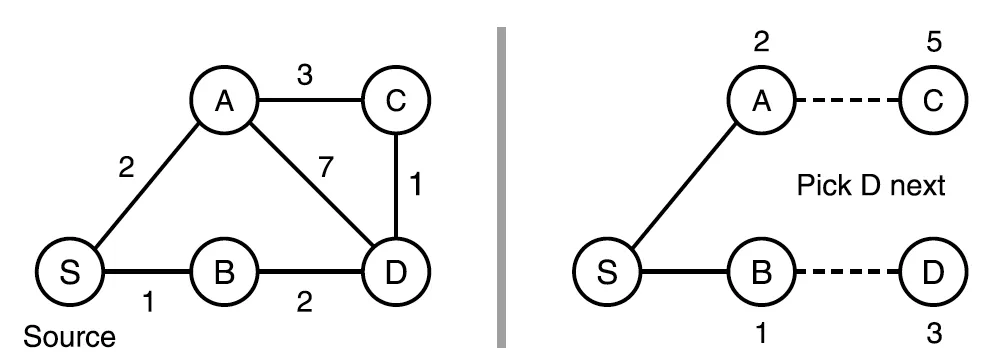
\includegraphics[width=0.8\textwidth]{../assets/ch01/ch01-1_2_网络算法学-009.png}
\end{figure}
图3.9显示，为了检索包含图像的网页，Web客户端通常必须发送一个GET请求以获取页面。如果页面指
定了内联图像，则客户端必须发送单独的请求以检索图像，然后才能显示页面。自然地，应用原则P1会
问，为什么需要单独的请求？为什么Web服务器不能在请求页面时自动下载图像，而不是等待单独的请
求？这应该至少减少一半的往返延迟。
为了测试我们的假设，我们修改了服务器软件以这样做，并测量了结果性能。令我们惊讶的是，我们发
现延迟仅略有改善。
使用基于tcpdump的网络分析器，我们发现了两个原因，说明这种看似改进的想法为何是一个坏主意。
 ● 与TCP的交互：Web传输由TCP协调，如第2章所述。为了避免网络拥塞，TCP从每次往返一个数据
   包开始缓慢增加其速率，然后在收到确认时增加到每次往返两个数据包，依此类推。由于TCP无论
   如何都必须等待确认以增加其速率，因此等待图像的额外请求并未增加延迟。
 ● 与客户端缓存的交互：许多客户端已经缓存了常见的图像，例如.gif文件。让Web服务器单方面下载
   客户端缓存中已有的图像是浪费带宽。请注意，客户端请求图像可以避免这个问题，因为客户端只
   会请求它没有的图像。
从这个案例研究中得到的有用教训是，由于与其他系统部分（如TCP拥塞控制）的交互，改进系统的一
部分可能很困难。
案例研究2：加速基于签名的入侵检测
作为第二个例子，许多网络站点部署了入侵检测系统，例如Snort（2001），它会查找数据包负载中表明
黑客攻击的可疑字符串。例如，字符串“perl.exe”可能表示试图执行perl并在Web服务器上执行任意命
令。对于每个可能匹配的规则，Snort使用Boyer-Moore算法（Cormen等，1990）分别搜索每个字符
串。最坏的情况是一个Web数据包匹配310条规则。简单的剖析使用gprof显示（Fisk和Varghese，
2001），Snort中30%的开销来自字符串搜索。
一个显而易见的应用原则P1似乎是：与其分别搜索每个字符串，不如使用一个集成的搜索算法，在一次
遍历数据包时搜索所有可能的字符串。我们修改了Boyer-Moore算法，使其成为一个集成的Boyer-
Moore算法，可以在一次遍历中搜索所有指定的字符串。在库中实现的新算法比Snort算法快50倍，适用
于完整的Snort数据库。不幸的是，当我们将它集成到Snort中时，我们发现几乎没有改进（Fisk和
Varghese，2001）。我们发现了两个原因。
 ● 多字符串匹配不是跟踪的瓶颈：对于给定的跟踪，很少有数据包匹配多个规则，每个规则包含单独


                                                      22
   的字符串。当我们使用仅包含Web流量（即目标端口为80的流量）的跟踪时，发现了显著的改进。
 ● 缓存效应：集成字符串搜索需要一个数据结构，例如trie，其大小随着被搜索的字符串数量的增长而
   增长。集成集合搜索的最简单方法是将所有规则中的字符串放在一个trie中。然而，当字符串数量超
   过100时，trie无法适应缓存，性能受到影响。因此，系统必须重新实现，以使用考虑硬件（P4）的
   较小集合。
从这个案例研究中得到的有用教训是，所谓的改进可能并未真正针对瓶颈（在跟踪中似乎是单字符串匹
配），并且可能与其他系统部分（数据缓存）发生交互。
3.5.1 八个警示性问题
本着这两个案例研究的精神，这里有八个警示性问题，提醒人们不要滥用这些原则。
Q1：是否值得提高性能？
如果将系统作为产品销售，性能是否是一个主要的卖点？关注性能改进的人可能希望如此，但系统的其
他方面，如易用性、功能性和稳健性，可能更为重要。例如，网络管理产品的用户更关心功能而非性
能。因此，在资源和实现复杂性有限的情况下，我们可能会选择推迟优化，直到需要时再进行。即使性
能很重要，哪个性能指标（例如，延迟、吞吐量、内存）是重要的？
在其他条件相同的情况下，简单性最好。简单的系统更容易理解、调试和维护。另一方面，简单性的定
义随着技术和时间的变化而变化。为了获得较大的性能提升，一定程度的复杂性是值得的。例如，多年
以来，像MPEG这样的图像压缩算法被认为过于复杂，无法在软件或硬件中实现。然而，随着芯片密度
的增加，许多MPEG芯片已经上市。
Q2：这真的是瓶颈吗？
80-20规则表明，大部分性能改进来自于优化系统中的一小部分。一个简单的开始方法是识别我们希望
优化的性能指标的关键瓶颈。一种方法是使用剖析工具，正如我们在案例研究2中所做的那样。
Q3：更改对系统其余部分有何影响？
一个简单的更改可能会加速系统的一部分，但可能对系统的其余部分产生复杂且不可预见的影响。这在
案例研究1中得到了说明。如果一个改进性能但与系统其他部分有太多交互的更改，应该重新考虑。
Q4：初始分析是否表明显著改进？
在进行完整实现之前，快速分析可以指示可能的增益。标准的复杂性分析是有用的。然而，当纳秒至关
重要时，常数因子也很重要。例如，假设分析表明路由器的地址查找是一个瓶颈（例如，因为有快速交

                                                  23
换机使数据传输不是瓶颈）。假设标准算法平均需要15次内存访问，而新算法的最坏情况为3次内存访
问。这表明有5倍的改进，这使得进一步进行变得有趣。
Q5：是否值得添加定制硬件？
随着通用处理器性价比的持续提高，人们很容易倾向于在软件中实现算法，并利用性价比曲线。因此，
如果我们正在考虑一块需要一年时间设计的定制硬件，并且结果的价格性能改进仅为2倍，那么可能不值
得付出努力。另一方面，随着有效的合成工具的出现，硬件设计时间正在缩短。批量生产也可以使定制
芯片的成本（与通用处理器相比）极低。在竞争激烈的市场中，即使只有一年的优势也是很有吸引力
的。这导致公司越来越多地将网络功能放在硅片中。
Q6：是否可以避免协议更改？
多年来，已经有许多提议谴责特定协议效率低下，并提出专门为性能设计的替代协议。例如，在20世纪
80年代，传输协议TCP被认为“慢”，并且明确设计为在硬件中实现的协议XTP（Chesson，1989）。这
激发了研究如何使TCP更快，最终在标准的BSD（Berkeley软件发行版）发布中，Van Jacobson实现了
TCP的快速实现（Clark等，1989）。最近，提出协议更改（例如，标签和流交换）以规避IP查找的需
求，激发了对快速IP查找的研究。
Q7：原型是否确认了最初的承诺？
一旦我们成功回答了所有前面的问题，仍然建议构建一个原型或模拟，并实际测试改进是否真实。这是
因为我们正在处理复杂系统；初始分析很少能捕捉到实践中遇到的所有效应。例如，理解Web图像转储
的想法不会改善延迟（见案例研究1），可能只有在实际实现并通过网络分析器进行测试后才会发现。
一个主要问题是找到一组标准基准测试，以比较标准和新的实现。例如，在通用系统领域，尽管存在一
些分歧，但存在用于浮点性能（例如，Whetstone）或数据库性能（例如，debit-credit）的标准基准测
试。如果有人声称通过差分编码减少Web传输延迟，那么提供一组合理的Web页面作为基准测试以证明
这一主张是什么？如果有人声称拥有一个小存储的IP查找方案，可以使用哪些基准数据库来支持这一断
言？
Q8：如果环境发生变化，性能提升是否会丧失？
即使构建了原型实现，并且基准测试表明性能改进接近初始预测，工作也尚未完成。困难在于，改进可
能特定于所使用的特定平台（可能会改变），并且可能利用了某个基准测试的属性（可能不反映系统将
使用的所有环境）。改进可能仍然是值得的，但某种形式的敏感性分析对于未来仍然有用。
例如，Van Jacobson对BSD网络代码进行了重大优化，使得普通工作站能够饱和100-Mbps FDDI（光
纤分布式数据接口）环。这种优化假设在正常情况下，下一个数据包来自与上一个数据包相同的连接P，
并且序列号比P高1。对于具有数千个同时连接到客户端的服务器，这种假设是否成立？如果数据包通过
                                                        24
网络中的并行链接发送，导致数据包重排序，这种假设是否成立？幸运的是，多年来代码运行良好。尽
管如此，这些问题提醒我们未来可能存在的危险。
3.6 总结
本章介绍了一套高效系统实施的原理。总结可以在图3.1-3.3中找到。这些原理通过从编译器、架构、数
据库、算法和网络中提取的示例进行了说明，以展示其对计算机系统的广泛适用性。Chef Charlie的示例
虽然有些戏谑，但表明这些原理也适用于从餐厅到州政府的通用系统。虽然广泛关注性能，但成本同样
是一个重要指标。可以将问题归结为在给定成本下找到最快的解决方案。优化其他指标（如带宽、存储
和计算）可以归入成本指标之下。
图3.1-3.3中的原理预览可以在后续章节中找到详细解释。前五个原则鼓励系统思维。接下来的五个原则
鼓励对系统模块化进行新的审视。最后五个原则指出了一些加速单个子系统的有用方法。
正如国际象棋策略在玩游戏之前是无聊的，实施原则在没有具体示例的情况下是毫无生气的。鼓励读者
尝试以下练习，这些练习提供了从计算机系统中提取的更多示例。其余章节将对这些原理在网络中的应
用进行探讨。特别是，下一章旨在通过提供一组15个独立的网络问题来吸引读者。


4 原则在行动
系统架构和设计就像任何艺术一样，只能通过实践来学习……只有在操作介质时，可能性的空间才会展
开。
——Carver Mead 和 Lynn Conway
在我把马群聚集起来之后，我现在开始让它们各展其能。——Arnold Toynbee
前一章概述了高效网络协议实现的15条原则。本书的第二部分开始详细研究特定的网络瓶颈，如数据复
制和控制转移。虽然这些原则在后续章节中也会用到，但这些章节的重点是所考察的具体瓶颈。鉴于网
络算法学既是一种思维方式，也是一套技术，通过在小型的、自成一体的但非平凡的网络问题上应用这
些原则来结束第一部分似乎是有用的。
因此，本章提供了在解决特定网络问题时应用这些原则的示例。这些示例来自真实问题，其中一些解决
方案已在实际产品中使用。与后续章节不同，本章不是一个新材料的集合，后面跟着一系列练习。相
反，本章可以被认为是一系列扩展的练习。
在4.1到4.15节中，描述了15个问题，并对每个问题进行了说明。每个问题后面都有一个提示，建议使用
特定的原则，然后是一个解决方案概述。每个解决方案后面还有一些练习。在关于本章主题的课程和研
讨会上，听众喜欢在得到一些提示后自己发明解决方案（而不是直接看到最终解决方案）。

                                                  25
快速参考指南
在一个理想的世界里，每个问题都应该对每个读者都有有趣的地方。然而，对于时间紧迫的读者，这里
有一些指导。硬件设计师如果想尝试一些问题，可以尝试设计一个以太网监控器（第4.4节）或对长标识
符进行二分搜索（第4.14节）。系统人员如果想了解系统思维如何巧妙地解决算法专业知识的问题，可以
尝试解决应用设备通道问题（第4.1节）或压缩连接表问题（第4.11节）。算法设计师可能会对识别资源
消耗者问题（第4.10节）和使用协议设计变更来简化链路状态路由中的实现问题（第4.8节）感兴趣。
4.1 应用设备通道的缓冲区验证
通常，应用程序只能通过操作系统内核发送网络数据，并且只有内核可以与网络适配器通信。这种限制
防止了不同应用程序恶意或意外地写入或读取彼此的数据。然而，通过内核进行通信会增加系统调用形
式的开销（见第2章）。在应用设备通道（ADCs）中，允许应用程序通过直接写入网络适配器的内存来
发送和接收网络数据。更多细节请参见第5章。一种无需内核调解的保护机制是让内核为每个应用程序设
置一组有效的内存页。然后，网络适配器必须确保应用程序的数据只能从有效页集合中的内存发送和接
收。
例如，在图4.1中，应用程序P被允许从有效页集合X、Y、...、L、A中发送和接收数据。假设应用程序P
向适配器发出请求，将下一个数据包接收到的缓冲区放入页A中。由于此请求是直接发送到适配器的，内
核无法检查这是否是P的有效缓冲区。相反，适配器必须通过确保A在有效页集合中来验证此请求。如果
适配器不执行此检查，应用程序P可能会提供一个属于其他应用程序的无效页，适配器会将P的数据写入
错误的页中。这种检查需求导致了以下问题。




In application device channels, the network adaptor is given a set of valid pages (X,Y,L,A, etc.)
for a given application P. When application P makes a request to receive data into page A, the
adaptor must check if A is in the valid list before allowing the receive.

                                                                                                    26
问题
当应用程序P执行接收操作时，适配器必须验证该页是否属于P的有效页集合。如果页集合被组织成一个
线性列表（Druschel等人，1994年），那么验证的成本为O(n)，其中n是集合中的页数。例如，在图4.1
中，由于A位于有效页列表的末尾，适配器必须在找到A之前遍历整个列表。如果n很大，这可能会非常
昂贵，并减慢适配器发送和接收数据包的速率。如何加快验证过程？
提示：减少验证复杂性的一个好方法是使用比列表更好的数据结构（P15）。你会选择哪种数据结构？然
而，通过系统思维并在接口中传递提示（P9），可以进一步改善最坏情况的行为并减小常数因子。
算法设计者会立即考虑将有效页集合实现为哈希表而不是列表。这提供了O(1)的平均搜索时间。哈希有两
个缺点：（1）具有小碰撞概率的好哈希函数在计算上代价昂贵；（2）哈希不提供良好的最坏情况界
限。二分搜索确实提供了对数最坏情况搜索时间，但如果页集合很大且数据包传输速率很高，这会很昂
贵（还需要保持集合有序）。相反，我们用索引数组查找替换哈希表查找，如下所示（在继续阅读之前
尝试使用P9）。
解决方案




Finessing the need for a hash table lookup by passing a handle across the interface between the
application and adaptor.
适配器将每个应用程序的有效页集合存储在一个数组中，如图4.2所示。这个数组只有在应用程序的有效
页集合被内核更新时才会更新。当应用程序请求将数据接收到页A时，它还会向适配器传递一个句柄
（P9）。该句柄是数组中存储A的位置的索引。适配器可以使用这个来快速确认接收请求中的页是否与
句柄中存储的页匹配。验证的成本是一个边界检查（查看句柄是否为有效索引）、一次数组查找和一次
比较。
练习
                                                                                             27
 ● 句柄是一个提示还是一个提示？让我们调用原则P1：如果这是一个句柄，为什么在接口中传递页号
   （例如A）？为什么在接口中移除页号可以稍微加快确认任务的速度？
 ● 通常需要使用哈希表搜索P来找到与应用程序P对应的数组。这削弱了摆脱哈希表搜索以检查页是否
   有效的论点——除非当然，P的哈希搜索也可以被巧妙地处理。如何做到这一点？
4.2 异步传输模式流量控制的调度器
在异步传输模式（ATM）中，ATM适配器可能有数百个同时的虚拟电路（VCs），这些虚拟电路可以发
送数据（称为信元）。每个VC通常以某种方式受到流量控制，以限制其发送速率。例如，在基于速率的
流量控制中，VC可能会在固定的时间间隔内接收发送信元的信用。另一方面，在基于信用的流量控制中
（Kung等人，1994年；Ozveren等人，1994年），当路径上的缓冲区释放时，下一个节点可能会发送信
用。




An ATM VC is eligible to send data if it is active (has some outstanding cells to send in the
queue shown below the VC) and has credits (shown by gray dots above the VC). The problem is
to select the next eligible VC in some fair manner without stepping through VCs that are
ineligible.
因此，在图4.3中，适配器有一个表，其中保存了VC的状态。已经建立了四个VC（1、3、5、7）。其
中，只有VC 1、5和7有一些信元要发送。最后，只有VC 1和7有信用可以发送信元。因此，适配器接下
来要发送的信元应该是来自符合条件的VC之一：1或7。从符合条件的VC中选择下一个信元应该公平地进
行，例如，以轮询的方式进行。如果适配器选择从VC 7发送一个信元，适配器会将VC 7的信用减少到
1。由于没有更多的信元要发送，VC 7现在变得不合格。选择下一个符合条件的VC会导致以下问题。
问题

                                                                                           28
一个简单的调度器可能会循环遍历VC数组，寻找一个符合条件的VC。如果许多VC都不符合条件，这可
能非常低效，因为调度器可能不得不遍历几个不符合条件的VC才能从一个符合条件的VC发送一个信元。
如何避免这种低效？
提示：考虑调用P12来添加一些额外的状态以加快调度器主循环的速度。你可以添加什么状态来避免遍历
不符合条件的VC？如何有效地维护这种状态？
解决方案




Maintaining a list of eligible VCs to speed up the scheduler main loop.
除了图4.3中的VC表之外，还维护一个符合条件的VC列表（图4.4）。唯一的问题是如何有效地维护这种
状态。这是使用P12的主要困难。如果状态维护成本过高，那么添加的状态就是一种负担而不是资产。回
想一下，VC符合条件是指它既有信元要发送又有信用。因此，VC在服务后如果没有信元要发送或没有更
多信用，就会从列表中移除；否则，VC会被添加到列表的尾部，以确保公平性。VC会在空VC信元队列
中到达一个信元并且这个（空的）队列也有信用，或者当VC没有信用并接收到信用更新时，被添加到列
表的尾部。
练习
 ● 如何确保一个VC不会被多次添加到符合条件的列表中？
 ● 这种方案是否可以推广，以允许某些VC根据管理者分配的权重获得比其他VC更多的发送机会？



4.3 使用Dijkstra算法进行路由计算
路由器S如何决定如何将数据包路由到给定目的地D？网络中的每条链路都被标记了一个成本，像S这样
的路由器通常会计算到本地域内目的地的最短（即最低成本）路径。假设成本是一个小整数。回想一下
第2章中提到的，在一个域内最常用的路由协议是基于链路状态路由的OSPF（开放最短路径优先）。
在链路状态路由中，子网中的每个路由器都会发送一个链路状态包（LSP），列出其与所有邻居的链路。
每个LSP都会被发送到子网中的每个其他路由器。每个路由器使用一个原始的洪泛协议（Perlman，1992
年）通过其LSP向其他路由器发送信息。一旦每个路由器从每个路由器接收到一个LSP，那么每个路由器
                                                                     29
就拥有了网络的完整地图。假设拓扑结构保持稳定，每个路由器现在可以使用标准的短路径算法（如
Dijkstra算法（Cormen等人，1990年））计算到网络中每个其他节点的最短路径。
在图4.5中，源S希望计算到网络中所有其他节点（A、B、C、D）的最短路径树。网络在图4.5的左框中
显示，链路编号带有其成本。在Dijkstra算法中，S首先将自己放入最短路径树中。S还会更新到达其直接
邻居（例如B、A）的成本。在每次迭代中，Dijkstra算法会将当前树中最接近的节点添加到树中。这个
新添加节点的邻居的成本会被更新。这个过程重复，直到网络中的所有节点都属于树。




In Dijkstra’s algorithm the source S builds a shortest-path tree rooted at S. At each stage, the
closest node not in the tree is added to the tree.
例如，在图4.5中，在添加S之后，算法选择B，然后选择A。在这次迭代中，树如图4.5右框所示。实线
显示了现有的树，虚线显示了到尚未在树中的节点的最佳当前连接。因此，由于A的成本为2，并且有一
条成本为3的链路从A到C，C被标记为5。类似地，D被标记为通过B的路径的成本为3。在下一次迭代
中，算法选择D作为尚未在树中的最小成本节点。然后使用通过D的路径更新C的成本。最后，在最后一
次迭代中，C被添加到树中。
这个教科书解决方案需要在每次迭代时确定一个不在树中的最小成本节点。跟踪动态变化集合中最小值
元素的标准数据结构是优先队列。这导致了以下问题。
问题
Dijkstra算法在N次迭代中需要一个优先队列，其中N是网络节点的数量。最好的通用优先队列，如堆
（Cormen等人，1990年），找到最小元素的成本为O(log N)。这意味着总运行时间为O(N log N)时间。
对于大型网络，这可能导致对故障和其他网络拓扑变化的响应缓慢。如何加快路由计算速度？
提示：考虑利用链路成本是小整数这一事实（P14），使用数组来表示节点的当前成本。如何有效地找到
下一个最小成本节点以包含在最短路径树中？
解决方案
可以利用链路成本是小整数这一事实来构建一个基于桶排序的优先队列（P14）。假设最大链路成本为
MaxLinkCost。因此，路径的最大成本不会超过Diam*MaxLinkCost，其中Diam是网络的直径。假设
                                                                                               30
Diam也是一个小整数。因此，可以想象使用一个数组，每个可能的成本c在范围1... Diam *
MaxLinkCost中都有一个位置。如果在Dijkstra算法的过程中节点X的成本从c变为c'，则节点X将从c的列
表中移除并添加到c'的列表中。但是如何找到最小元素呢？这可以通过初始化一个名为CurrentMin的指
针来实现，指向0（对应于S的成本）。每次算法希望找到不在树中的最小成本节点时，CurrentMin递增
1，直到到达一个包含非空列表的数组位置。然后可以将该列表中的任何节点添加到树中。算法的成本为
O(N + Diam * MaxLinkCost)，因为在推进CurrentMin时最多只能进行数组大小的操作。对于大型N和
小Diam和MaxLinkCost值，这可能比N log N要好得多。
能够有效使用前面描述的基于桶排序的优先队列的一个关键因素是，节点成本始终领先于CurrentMin的
值。这是一个单调性条件。如果不是这样，算法将在每次迭代时从1开始检查最小值，而不是从上一次
CurrentMin的值开始，并且永远不会回退。对于Dijkstra算法来说，这个单调性条件是相当明显的，因为
尚未在树中的节点的成本必须大于已在树中的节点的成本。




Using a priority queue based on bucket sorting to speed up Dijkstra’s algorithm.
图4.6显示了在A被添加到树中之后基于桶排序优先队列的状态。这对应于图4.5的右框。此时，
CurrentMin=2，这是A的成本。在下一次迭代中，CurrentMin将递增到3，D将被添加到树中。这将导致
C的成本降低到4。因此，我们将C从位置5的列表中移除，并将其添加到位置4的空列表中。然后
CurrentMin递增到4，C被添加到树中。
练习
 ● 如何有效地将一个节点从一个列表中移除并添加到另一个较早的列表中？
 ● 在图4.6中，算法如何知道在将C添加到树中后可以终止，而不是推进到长数组的末尾？
 ● 在实际网络中，故障会导致直径发生很大变化，因为故障可能会显著增加网络的直径。例如，在一
   个轮式拓扑中，所有N个节点通过一个中心辐条节点的直径为2；如果中心辐条节点发生故障，直径
   将增加到N/2。实际上，直径通常很小。这是否会导致在确定数组大小时出现问题？
 ● 是否可以通过用大小为MaxLinkCost的循环数组替换图4.6中的线性数组来完全规避直径问题？解释
   一下。这种解决方案被称为Dial算法（Ahuja等人，1993年）。

                                                                              31
4.4 使用桥接硬件的以太网监控器
Alyssa P. Hacker 在 Acme Networks 工作，她知道 Acme 发明的以太网桥。桥是一种可以连接以太网
的设备。为了将数据包从一个以太网转发到另一个以太网，桥必须以高速度在以太网数据包中查找48位
目标地址。
Alyssa 决定将桥改造成一个以太网流量监控器，该监控器将被动监听以太网并生成有关流量模式的统计
信息。营销人员告诉她，她需要监控任意源-目的地址对之间的流量。因此，对于每对活动的源-目的地
址对，如A、B，Alyssa必须维护一个变量PA,B，用于测量自监控器启动以来从A发送到B的数据包数量。
当从A发送到B的数据包到达时，监控器（监听电缆上发送的所有数据包）将捕获数据包的副本。如果源
是A且目的地是B，监控器应增加PA,B。问题在于如何在64微秒内完成这一任务，这是以太网上最小数据
包间隔时间。瓶颈在于查找与一对48位地址A、B相关联的状态PA,B。
幸运的是，桥接硬件具有一个出色的查找硬件引擎，可以在1.4微秒内查找单个48位地址的状态。可以表
示为Lookup(X,D)，其中X是48位键，D是要搜索的数据库。调用将在1.4微秒内返回与X相关联的状态，
适用于少于64,000个键的数据库。Alyssa需要解决以下问题。
问题
监控器需要在从A到B的数据包到达时更新PA,B的状态。监控器有一个只能查找单个地址的查找引擎，而
不是地址对。Alyssa如何使用现有的引擎来查找地址对？问题如图4.7所示。




Adapting an engine that does destination lookups to doing source-destination lookups
提示：问题要求利用现有的桥接硬件（P4c）。由于1.4微秒远小于64微秒，设计可以承担多个硬件查找
的成本。如何使用三个查找将96位查找转换为48位查找？
一个简单的解决方案是使用两个查找将源A和目的地B转换为较小的（<24位）索引IA和IB。然后可以使
用这两个索引来查找存储AB状态的二维数组。这只需要两个硬件查找加上一次内存访问，但可能需要大
量内存。如果可能有20,000个活动的源-目的地址对，而只有1000个可能的源和1000个可能的目的地，
那么数组必须包含一百万个条目。如何使所需的内存量与实际活动的源-目的地址对的数量成正比？


                                                                                   32
解决方案
如前所述，首先使用一次查找将源A和目的地B分别转换为较小的（<24位）索引IA和IB。然后使用第三
次查找将IA和IB映射到AB状态。解决方案如图4.8所示。第三次查找有效地压缩了简单解决方案中的二维
数组。这个解决方案是由Mark Kempf和Mike Soha提出的。




Converting a 96-bit lookup into a 48-bit lookup by first converting each 48-bit address into a
24-bit index and concatenating the indices.
练习
 ● 是否可以使用仅两个桥接硬件查找而不需要额外的内存来解决这个问题？
 ● 活动的源-目的地址对可能会随着时间的推移而变化，因为某些地址对可能在很长一段时间内停止通
   信。如何在不保留自监控器启动以来所有通信过的地址对的每个可能地址对的状态的情况下处理这
   种情况？
4.5 x-kernel中的解复用
x-kernel（Hutchinson和Peterson，1991年）提供了一个用于主机协议实现的软件基础设施。x-kernel
系统支持许多必需的协议功能。一个常见的必需功能是协议解复用。例如，当互联网路由层IP接收到一
个数据包时，它必须使用协议字段来确定数据包接下来应该发送到TCP（传输控制协议）还是UDP（用
户数据报协议）。
大多数协议确实基于协议头中的某个标识符进行解复用。这些标识符在不同的协议中可以有不同的长
度。例如，以太网类型字段可以是5字节，而TCP端口号是2字节长。因此，x-kernel允许基于可变长度
协议标识符进行解复用。当系统初始化时，协议例程可以向x-kernel注册标识符与目标协议之间的映
射。运行时，当数据包到达时，协议例程可以从数据包中提取协议标识符，并查询x-kernel解复用例程
以获取目标协议。由于数据包可能以高速到达，解复用例程应该快速。这导致了以下问题。
问题
                                                                                                 33
通常，最快的查找方法是使用哈希表。如图4.9所示，这需要对标识符K进行某种哈希函数计算以生成哈
希索引，使用该索引访问哈希表，并将存储在哈希表条目中的键L与K进行比较。如果匹配，则解复用例
程可以检索与键L相关联的目标协议。假设已经选择了哈希函数以使冲突不频繁。




Demultiplexing in the x-kernel is done by hashing the protocol identifier K and (potentially) using
a byte-by-byte comparison with the key L stored at the hash table entry.
然而，由于标识符的长度是任意数量的字节，比较例程通常必须逐字节进行比较。但是，假设最常见的
情况是4字节标识符，这是机器字的大小。在这种情况下，使用字比较会更高效。因此，目标是利用高效
的字比较（P4c）来优化预期情况（P11）。如何在仍然处理任意协议的同时做到这一点？
提示：注意，如果x-kernel需要解复用一个3字节标识符，它必须使用逐字节比较例程；如果x-kernel需
要解复用一个4字节标识符，并且4字节是机器字大小，它可以使用字比较。第一个可以利用的自由度是
为最常见的情况（例如，字比较、长字比较）提供不同的比较例程，并为每种协议提供一个默认的比较
例程，该例程使用逐字节比较。这样做是以额外的空间换取时间（P4b）。然而，为了正确性，了解每种
协议应使用哪种比较例程是很重要的。考虑调用原则P9在接口中传递提示和P2a进行一些预计算。
解决方案
每个协议在系统初始化时都必须向x-kernel声明其标识符和目标协议。此时，每个协议都可以预先声明
其标识符长度，因此x-kernel可以为每个协议使用专门的比较例程。实际上，信息是在客户端协议和x-
kernel之间传递的（P9），并且在早期（P2a）进行。假设x-kernel为每个客户端协议都有一个单独的哈
希表，并且x-kernel知道每个客户端的上下文，以便使用该客户端的专用代码。
练习
 ● 在你的机器上编写字节逐字节和字比较的代码，并进行大量两种类型的比较，比较每种类型的总体
   时间。
 ● 在早期的ADC解决方案中，通过传递索引（而不是标识符长度）来简化哈希表查找。为什么在这种
   情况下这种方法可能比较困难？
4.6 带节点压缩的Trie树
                                                                                                34
Trie storing three keys. Notice the wasted space in the trie nodes.
Trie是一种树形数据结构，其中每个节点是一个包含M个元素的数组。\begin{figure}[htbp]
\centering
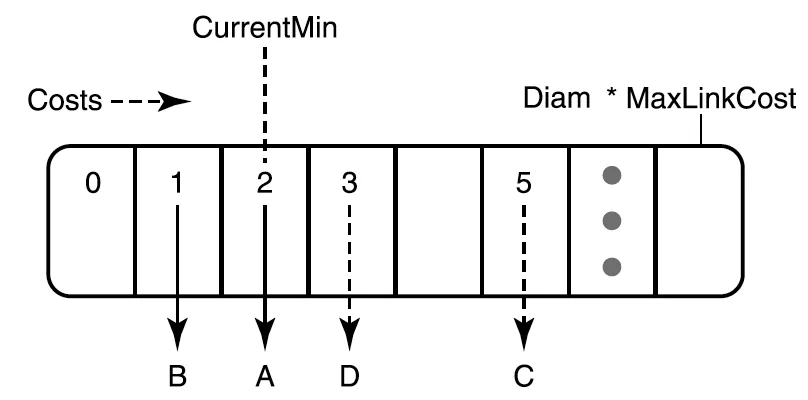
\includegraphics[width=0.8\textwidth]{../assets/ch01/ch01-1_2_网络算法学-010.png}
\end{figure}
图4.10展示了一个简单的例子，
M=8。每个数组可以存储一个键（例如，图4.10中的KEY 1、KEY 2或KEY 3）或指向另一个Trie节点的
指针（例如，图4.10顶部Trie节点的第一个元素，即根节点）。Trie用于搜索输入字符串的精确匹配（和
最长前缀匹配）。在网络中，Trie用于各种任务，如IP地址查找（第11章）、桥接查找（第10章）和解复
用过滤器（第8章）。
具体的Trie算法在这里并不重要。我们只需要知道如何搜索Trie。设 c = log2 M 为Trie的块大小。为
了搜索Trie，首先将输入字符串分成大小为c的块。搜索从最高有效位开始，使用连续的块来索引Trie的
                                                  ​




节点，从根节点开始。当搜索使用块j索引当前Trie节点的位置i时，位置i可以包含一个指针或一个键。如
果位置i包含一个非空指针到节点N，则搜索继续在节点N中使用块j+1；否则，搜索终止。
总结来说，每个节点是一个指针或键的数组，搜索过程需要索引这些数组。然而，如果许多Trie节点是稀
疏的，就会浪费大量空间（P1）。例如，在图4.10中，16个位置中只有4个包含有用信息。在最坏的情况
下，每个Trie节点可能包含1个指针或键，并且可能存在M倍的浪费内存。假设 M ≤ 32 ，即使M这么
小，也可能导致内存增加32倍，这会大大增加设计成本。
一个显而易见的解决方案是用线性列表替换每个Trie节点，形式为(i, val)，其中val是节点中位置i的非空
值（指针或键）。例如，图4.10中的根Trie节点可以被替换为列表 (1, ptr1); (7, KEY 1) ，其中ptr1
是指向底部Trie节点的指针。不幸的是，这可能会使Trie搜索速度减慢M倍，因为每个Trie节点的搜索可
能现在需要在M个位置的列表中进行搜索，而不是单个索引操作。这导致了以下问题。
问题
如何压缩Trie节点以去除空指针而不显著减慢搜索速度？
提示：尽管压缩了节点，数组索引仍需高效。如果节点被压缩，如何表示哪些数组元素被移除的信息？
考虑利用M较小这一事实（P14和P4a）。
解决方案
                                                                 35
由于 M < 32 ，一个大小为32的位图可以轻松地放入一个计算机字中（P14和P4a）。因此，在添加了
一个位图后，空指针被移除，位图中零位表示原始位置的空指针。如\begin{figure}[htbp]
\centering
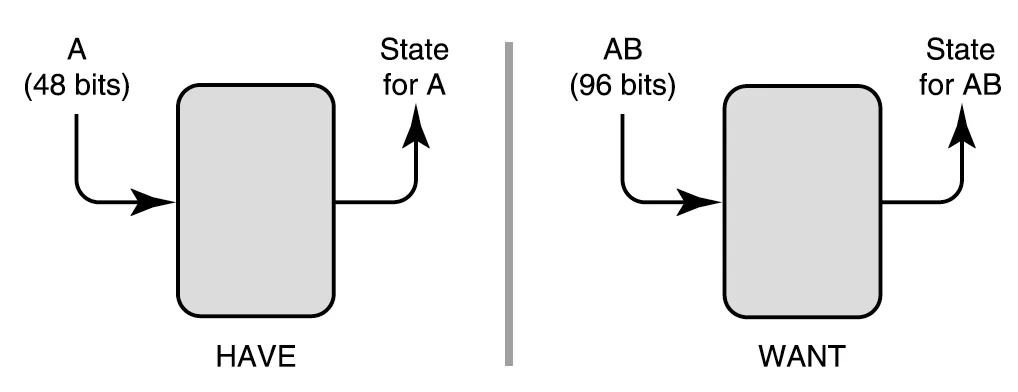
\includegraphics[width=0.8\textwidth]{../assets/ch01/ch01-1_2_网络算法学-011.png}
\end{figure}
图4.11所示，Trie节点现在可以被替
换为一个位图和一个压缩的Trie节点。压缩的Trie节点是一个仅包含原始节点中非空值的数组。因此，在
图4.11中，原始根Trie节点（顶部）已被替换为压缩的Trie节点（底部）。位图在第一个和第七个位置包
含1，表示根节点包含非空值。压缩后的数组现在只包含两个元素，第一个指针和KEY 3。这仍然引出了
一个问题：如何搜索Trie节点？




Compressing a trie node using a bitmap and bit counting to efficiently translate from an
uncompressed index to a compressed index.
由于未压缩和压缩的节点都是数组，并且搜索过程从索引I开始进入未压缩节点，搜索过程必须咨询位图
以将未压缩索引I转换为压缩索引C进入压缩节点。例如，如果I是1，则C应该是1；如果I是7，则C应该是
2。如果I是其他值，则C应该是0，表示只有一个空指针。
幸运的是，从I到C的转换可以通过以下方式轻松完成。如果位图中的位置I包含0，则C=0。否则，C是位
图中前I位中1的数量。因此，如果 I = 7 ，则 C = 2 ，因为位图中的前七位中有两个位被设置。
练习
 ● 如何使用表查找（P14，P2a）来加速软件中计算位图中1的数量？这是否一定需要第三次内存引用？
 ● 假设位图很大（例如， M = 64K ）。在硬件或软件中计算这样一个大位图中1的数量似乎慢得不
   可思议。你能找到一种方法，仅使用一次额外的内存访问来加速大位图中1的计算吗？这在第11章中
   将非常有用。
4.7 路由器中的数据包过滤

                                                                                      36
第12章描述了在路由器上设置资源以处理需要性能保证的流量（如视频）的协议。这些协议使用数据包
过滤器的概念，有时称为分类器。因此，在\begin{figure}[htbp]
\centering
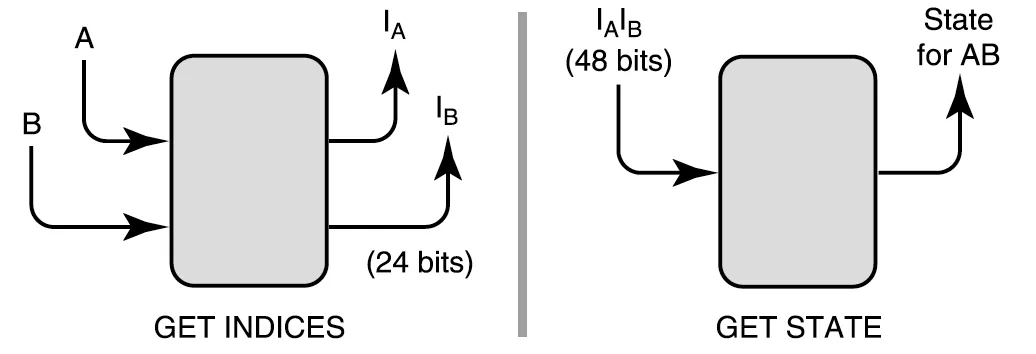
\includegraphics[width=0.8\textwidth]{../assets/ch01/ch01-1_2_网络算法学-012.png}
\end{figure}
图4.12中，连接到路由器的每个接收器可能指定一个数据包过
滤器，描述其希望接收的数据包。例如，在图4.12中，接收器1可能希望接收NBC，这由过滤器4指定。
每个过滤器都是对NBC发送的视频数据包的字段的某种规范。例如，NBC可能由使用德国NBC发射机的
源地址和指定的TCP目标和源端口号的数据包指定。
同样，在图4.12中，接收器m可能希望接收ABC Sports和CNN，这分别由过滤器1和7描述。数据包以高
速到达路由器，并且必须发送给所有请求该数据包的接收器。例如，接收器1和2可能都希望接收NBC。
这导致了以下问题。




Packet filtering in a router may require a slow linear scan of all filters followed by making a copy
of the packet for all filters that match.
问题
每个到达的数据包必须与所有过滤器匹配，并发送给所有匹配的接收器。如果过滤器数量很大，简单的
线性扫描所有过滤器会很昂贵。假设过滤器数量超过一千。如何加快这一昂贵的过程？
提示：人们可能会考虑通过缓存（P11a）来优化预期情况。然而，为什么在这种情况下缓存很困难？考
虑在数据包头中添加一个字段（P10），以使缓存更容易。理想情况下，这个字段应该添加到哪个协议
层？添加一个不需要全局标准化标识符的固定众所周知的字段对于每个可能的视频类型是不够的，因为
过滤器可能基于其他字段，如源地址。假设你添加的字段不需要全局标准化的标识符。发送方必须确保
什么？
解决方案
缓存（P11a），系统设计师的老工具，在这个问题上并不十分直接。通常，缓存存储输入a和某些输出
f(a)之间的映射。然后，缓存由形式为(a,f(a))的对组成。这些对存储在一个数据库中，以a的值作为键。
该数据库可以实现为一个哈希表（在软件中）或内容可寻址存储器（在硬件中）。给定输入a并需要计算
                                                                                                   37
f(a)，首先检查数据库中是否存在a。如果存在，则快速路径退出并返回现有的f(a)。如果不存在，则使用
某种（可能昂贵的）计算来计算f(a)，并将对(a,f(a))插入缓存数据库。随后具有值a的输入可以非常快速
地计算。
在数据包过滤问题中，目标是计算与数据包P相关联的接收器集合。问题是输出是P的（可能很大的）数
据包头字段集合的函数。因此，要使用缓存，必须存储P的头部的大部分与接收器集合的映射。存储64字
节数据包头部与接收器集合的映射是一个昂贵的提议。这在时间上昂贵，因为搜索缓存可能需要更长时
间，因为键很宽。这显然在存储上也昂贵。更大的存储需求反过来意味着给定缓存大小可以缓存的映射
更少，这导致缓存命中率较低。
理想的情况是缓存一个或两个数据包字段与输出接收器集合之间的映射。这将加快缓存搜索速度并提高
缓存命中率。这些字段最好也在路由头中，路由器无论如何都会检查这些字段。问题是可能没有这样一
个唯一指纹数据包P的字段。
然而，假设我们是设计路由协议的设计师。我们可以向路由头添加一个字段。问题似乎很简单，如果我
们可以为每个可能的流分配一个唯一的全球标识符。例如，如果我们可以为NBC分配标识符1，为ABC分
配标识符2，为CNN分配标识符3，那么我们可以使用标识符作为键进行缓存。这样的解决方案将需要某
种全球标准委员会负责命名每个应用流。即使这可以实现，接收器过滤器可能要求所有NBC数据包来自
某个源，并且过滤器可能依赖于其他数据包字段。这导致了以下最终想法。




Adding a flow identifier (which is unique only with respect to a source) can speed up packet
filtering.
更改路由头以添加一个流标识符F（\begin{figure}[htbp]
\centering
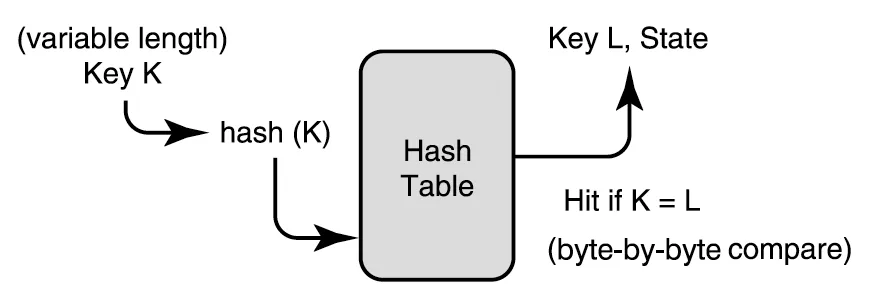
\includegraphics[width=0.8\textwidth]{../assets/ch01/ch01-1_2_网络算法学-013.png}
\end{figure}
图4.13），其含义取决于源。换句话说，不同的源可以使用相同的流
标识符，因为是源和流标识符的组合是唯一的。因此，不需要全球标准化（或其他全球协调）流标识
                                                                                          38
符。流标识符只是源维护的一个本地计数器。想法是发送应用程序可以向路由层请求一个流标识符。这
个标识符被添加到该应用程序所有数据包的路由头中。
通常，当应用程序数据包第一次到达时，路由器会进行（缓慢的）线性搜索，以确定与数据包头相关联
的接收器集合。由于标识符在源之间不唯一，路由器会缓存使用源地址和流标识符的连接作为键的映
射。显然，正确性取决于发送应用程序在不更改可能影响过滤器的数据包字段的情况下不更改数据包中
的流标识符。
练习
 ● 如果源崩溃并在没有记住它为不同应用程序分配了哪些标识符的情况下重新启动，会发生什么？当
   接收器添加新过滤器时会发生什么？如何解决这些问题？
 ● 在当前解决方案中，流标识符被用作提示（第3章），而不是提示。如果将流标识符-源地址对视为
   提示而不是提示，会带来哪些额外成本？
4.8 避免LSP的碎片化
以下问题实际上出现在OSI和OSPF（Perlman，1992年）链路状态路由协议的设计过程中。这个问题是
关于协议设计的，而不是协议实现（一旦设计确定）。尽管如此，它说明了设计选择如何极大地影响实
现性能。
第2章和第4.3节描述了链路状态路由。回想一下，在链路状态路由中，路由器必须发送一个LSP，列出
其所有邻居。链路状态协议包括两个独立的过程。第一个是更新过程，它使用依赖于每个LSP的唯一序列
号的可靠洪泛协议从一个路由器向另一个路由器发送LSP。序列号用于拒绝重复的LSP副本。每当路由器
从源S接收到编号为x的新LSP时，路由器将记住编号x，并拒绝来自S的任何后续具有序列号x的LSP。在
更新过程完成其工作后，每个路由器上的决策过程将应用Dijkstra算法到由LSP形成的网络图。
虽然路由器可能只有少量路由器邻居，但路由器可能有大量直接连接到同一局域网的主机计算机（端节
点）。例如，在\begin{figure}[htbp]
\centering
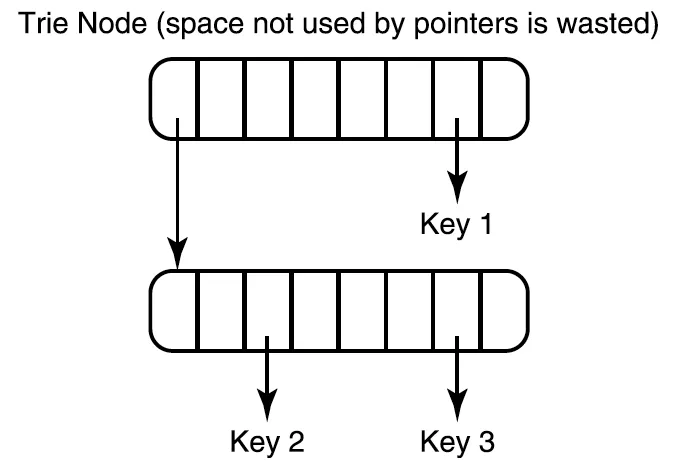
\includegraphics[width=0.8\textwidth]{../assets/ch01/ch01-1_2_网络算法学-014.png}
\end{figure}
图4.14中，路由器R1有500个端节点邻居E1...E500。大型局域网甚至可能有更多的端节
点。这导致了以下问题。




                                                    39
The LSP of router R1 (with even 500 endnode neighbors) may be too large to fit into a data link
frame. Without a clever idea, this would require inefficient fragmentation and reassembly of the
LSP at every hop.
问题
每个端节点占用8字节（6字节用于标识端节点，2字节用于成本信息），LSP可能会非常大（对于5000
个端节点为40,000字节）。这对于许多常用数据链路上的最大帧大小来说太4.15大了。例如，以太网的
最大帧大小为1500字节，FDDI指定最大帧大小为4500字节。这意味着大LSP必须在每个跃点上被分割成
许多数据链路帧，并在每个路由器上重新组装后才能继续发送。这需要在每个跃点上进行昂贵的重新组
装过程，以确定是否已接收到LSP的所有部分。
这还会增加链路状态传播的延迟。假设每个LSP可以装入M个数据链路帧，网络的直径为D，发送数据链
路帧的时间为1个时间单位。那么，使用逐跳重新组装时，LSP的传播时间为D·M。如果路由器不必在每
个跃点等待重新组装每个LSP，则传播延迟仅为M+D。当设计链路状态协议时，实现者发现了这些问题
（Perlman，1992年）。
另一方面，似乎不可能独立传播片段，因为LSP携带一个对更新过程至关重要的单一序列号。简单地将序
列号复制到每个片段中是无济于事的，因为这将导致后续片段被拒绝，因为它们具有与第一个片段相同
的序列号。问题是使不可能成为可能，通过空间上的计算转移来避免逐跳碎片化。允许对LSP路由协议进
行更改。
提示：所有5000个端节点的信息是否必须位于同一个LSP中？考虑调用P3c来转移空间上的计算。
解决方案
如果原始R1的LSP的各个片段要独立传播而不进行逐跳重新组装，则每个片段必须是一个单独的LSP，并
具有单独的序列号。这个关键观察导致了以下巧妙的方法。




Avoiding hop-by-hop fragmentation by dividing a large router into pseudorouters.

                                                                                                   40
修改链路状态路由协议，允许任何路由器R1成为多个伪路由器R1a、R1b、R1c（见\begin{figure}[htbp]
\centering
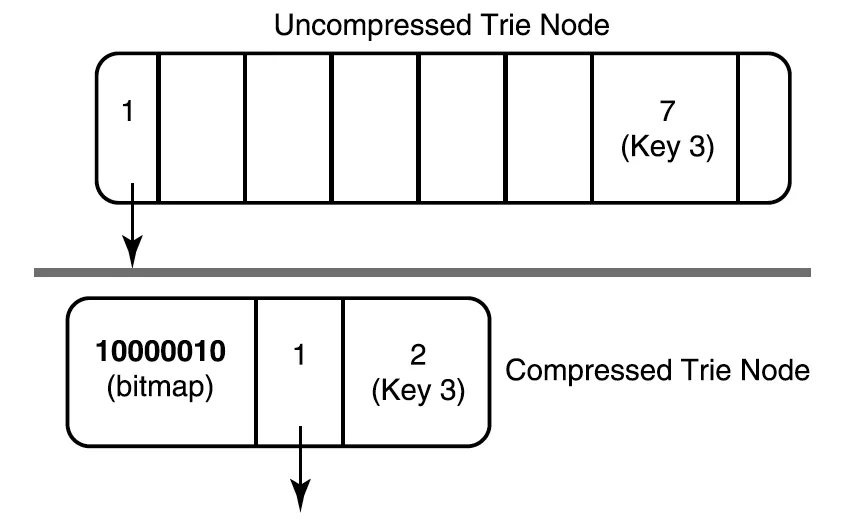
\includegraphics[width=0.8\textwidth]{../assets/ch01/ch01-1_2_网络算法学-015.png}
\end{figure}
图4.15）。原始的端节
点集合被分配到这些伪路由器中，因此每个伪路由器的LSP可以装入大多数数据链路帧而无需碎片化。例
如，如果大多数数据链路大小至少为576字节，则大约72个端节点可以装入一个数据链路帧。
如何实现伪路由器的概念？在原始LSP传播中，每个路由器都有一个6字节的ID，放置在所有由该路由器
发送的LSP中。为了允许伪路由器，我们更改协议，使LSP携带一个7字节ID（6字节路由器ID + 1字节伪
路由器ID）。伪路由器ID可以由实际包含所有伪路由器的路由器分配。通过允许每个路由器有256个伪路
由器，大约18,000个端节点可以支持每个路由器。
虽然LSP传播将伪路由器视为单独的实体，但重要的是路由计算将不同的伪路由器视为同一个路由器。毕
竟，端节点都直接连接到R1。但这很容易做到，因为所有以相同前6字节开头的LSP都可以被识别为来自
同一个路由器。
总之，主要思想是通过让源将原始LSP碎片化为独立的LSP来转移空间上的计算（P3c），而不是让每个
数据链路进行碎片化。这是一个很好的系统思维示例。不用说，实现者比原始方法更喜欢这个解决方案
（由Radia Perlman发明）。
练习
● 路由器如何分配端节点到伪路由器？如果路由器最初有很多端节点（因此有很多伪路由器），然后
  大多数端节点死亡，会发生什么？这可能会留下许多伪路由器，每个伪路由器只有少数端节点。为
  什么这不好，如何解决？
● 如第3章中描述的放宽一致性示例一样，这种解决方案可能导致一些意外的（但不是很严重的）临时
  不一致。假设解决了前面的练习，描述一个场景，在该场景中，某个路由器（例如R2）可能会在某
  个时刻发现其LSP数据库显示同一个端节点（例如E1）属于两个伪路由器R1a和R1c。为什么这比普
  通的LSP路由更糟糕？
4.9 流量模式监管
一些网络协议要求源在特定时间段T内发送的数据不超过一定速率。协议可能不仅指定长时间内的平均速
率（如B/T比特每秒），还指定用户在任何T秒时间段内可以发送的最大流量B比特。这确实将源限制在
平均速率为B/T比特每秒。然而，它也将用户的“突发性”流量限制为每个T时间段内最多一个大小为B的
突发。例如，选择较小的T值可以大大限制流量的突发性。突发性会给网络带来问题，因为高流量和数据
包丢失的时期之后是空闲时期。
如果每个源都遵守其合同（即，在指定时间段内发送不超过指定数量的数据），网络通常可以保证性
能，并确保没有流量被丢弃，并且所有流量都能及时交付。不幸的是，这就像说如果每个人都遵守交通
规则，交通就会顺畅流动。大多数人确实遵守规则：有些人因为觉得这是正确的事情，而许多人则是因
为他们知道如果被交通警察抓住会面临处罚。因此，监管是有序社会的重要组成部分。

                                                   41
简单地使用单个或多个计时器（检查流量是否在每个T秒时间段内发送不超过B比特）并不能捕捉到所有
违规行为。
出于同样的原因，许多设计者主张网络应定期监管流量，以查找不符合其合同的违规者。如果没有监
管，违规者可以获得不成比例的网络带宽份额。
假设路由器需要确保特定流量流在T秒时间段内不超过B比特。最简单的解决方案是路由器使用一个每T
秒滴答一次的单个计时器和每个流的计数器。在每个时间段结束时，如果计数器超过B，则检测到违规行
为。
不幸的是，单个计时器只能监管某些时间段。例如，假设不失一般性地计时器从时间0开始滴答。那么唯
一检查的时间段是[T,2T],[2T,3T],.... 这并不能确保源流在重叠的时间段（如[T/2,3T/2]）内不违反其合
同。
例如，在\begin{figure}[htbp]
\centering
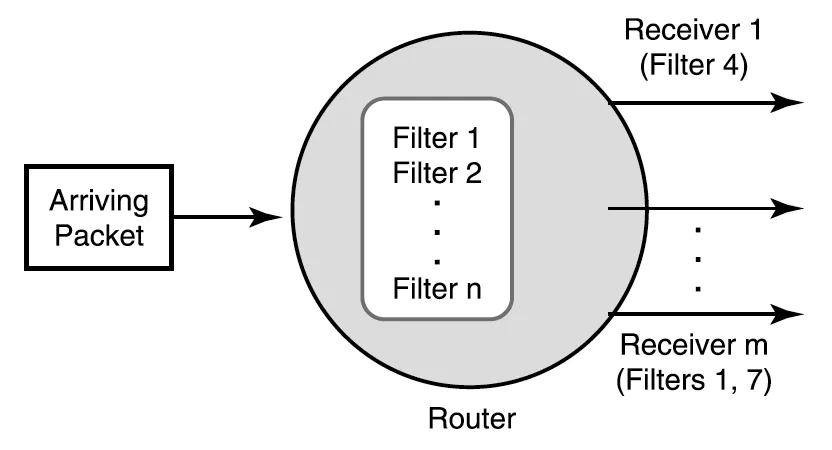
\includegraphics[width=0.8\textwidth]{../assets/ch01/ch01-1_2_网络算法学-016.png}
\end{figure}
图4.16的左侧框架中，流量在T之前的瞬间发送一个大小为B的突发，并在T之后的瞬间发送第二
个大小为B的突发，从而在一个略大于T/2的时间段内发送2B。




The naive use of a single or multiple timers (to check whether a flow sends no more than B every
T seconds) does not catch all violations.
不幸的是，两个计时器都无法检测到流量作为违规者。这种流量可以通过在每个被监管的时间段内发送
不超过B比特的数据来避免被检测为违规者，但在某些重叠的时间段内可能会发送超过B比特的数据。
为了解决这个问题，可以尝试使用多个计时器和计数器。例如，路由器可以使用一个从0开始的计时器和
另一个从T/2开始的计时器。然而，流量仍然可以通过在每个被监管的时间段内发送不超过B比特的数据
来规避检测，同时在某些重叠的时间段内发送超过B比特的数据。例如，在图4.16的右侧框架中，违规流
量在第一个时间段的末尾发送一个大小为B的突发，然后在第三个时间段的开始发送第二个大小为B的突
发，从而在一个略大于T/2的时间段内发送了2B。然而，这两个计时器都无法检测到该流量作为违规
者。
因此，需要一种更有效的方法来检测违规流量。可以考虑利用一些自由度（P13），这些自由度在简单解
决方案中被假定为固定的。是否需要固定监管间隔的开始时间？此外，考虑使用P3a。

                                                                                              42
解决方案
如提示所建议的，监管间隔不需要固定。因此，可以在计时器滴答之间设置任意的时间间隔。应该如何
选择这个间隔呢？由于违规流量可以选择在任何时刻开始其违规时间段T，一个简单的想法是引入以下概
念：
路由器使用一个T单位的计时器和一个计数器，如前所述。当计时器滴答时，如果计数器大于B，则检测
到违规行为。然后设置一个标志，指示计时器现在仅用于插入一个随机间隔。然后，计时器重新启动，
随机时间间隔在0到T之间。当计时器滴答时，清除标志并初始化计数器，并将计时器重置为T单位的时间
以开始下一次监管。
通过这种方式，违规流量无法预测监管间隔的开始时间，从而增加了被检测到的概率。
练习
● 假设计数器在间隔期间也被初始化和维护，即使在监管间隔之外的间隙期间也是如此。路由器能否
  在间隙期间做出任何有效的推断，即使间隙期间小于T单位？
● （开放问题）假设流量是有对抗性的。流量如何制定一个策略，以尽可能高地违反合同并仍然逃避
  前面描述的随机检测器的检测？流量策略可以是随机的。一个好的答案应该通过概率分析来支持。
4.10 识别资源消耗大户
假设一个设备希望跟踪各种用户的资源消耗情况，例如路由器分配给各个源的数据包内存。该设备需要
一种廉价的方法来找到消耗最多资源的用户，以便可以从这样的资源消耗大户那里回收内存。\begin{figure}[htbp]
\centering
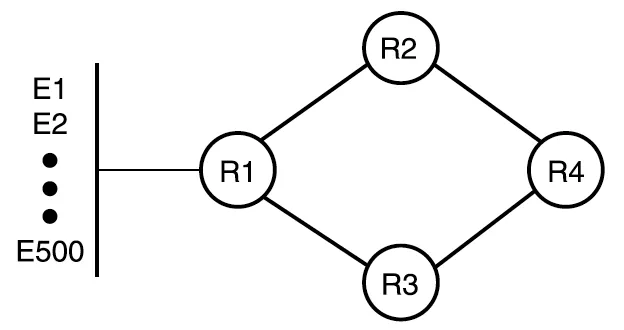
\includegraphics[width=0.8\textwidth]{../assets/ch01/ch01-1_2_网络算法学-018.png}
\end{figure}
图4.18显示
了五个源及其当前的资源消耗量分别为1、9、30、24和7个单位。资源消耗大户是S3。
问题
一个简单的解决方案是使用堆。然而，如果源的数量超过一千，这在高速情况下可能代价过高。假设描
述资源使用的数字是1到8000之间的整数。因此，桶排序技术可能不太适用，因为我们可能需要搜索
8000个条目才能找到资源消耗大户。
假设设备不关心确切的最大值，只要结果在2倍以内即可（P3b中提到的完美公平性不重要）。例如，在
图中，假设得到24而不是30是可以接受的。这种对准确性要求的放宽能否转化为更高效的算法？
提示：考虑使用三个原则：通过交易准确性来减少计算量（P3b）、使用桶排序（P14）和使用表查找
（P4b，P2a）。
解决方案
                                              43
由于结果可以在2倍以内，将资源消耗在2倍以内的用户聚合到同一个“资源消耗组”是有意义的。如果结
果组的数量比原始用户数量小得多，那么找到最大组将比找到最大用户更快。这类似于分层路由中的聚
合概念，其中多个目的地被聚合在一个共同的前缀下；这可能会使路由不够精确，但减少了路由条目的
数量。这导致了以下思路（在继续阅读之前尝试自己理清细节）。
可以使用二项式桶排序，如\begin{figure}[htbp]
\centering
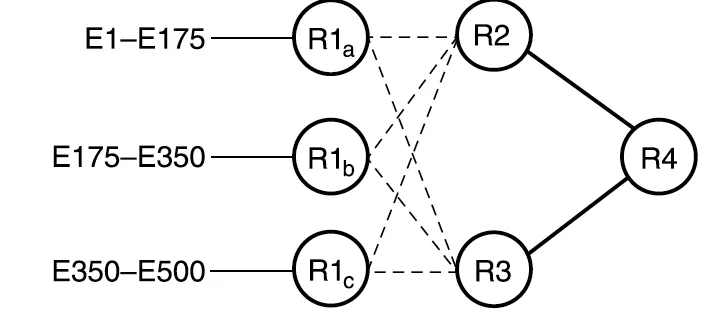
\includegraphics[width=0.8\textwidth]{../assets/ch01/ch01-1_2_网络算法学-019.png}
\end{figure}
图4.19所示，所有用户根据资源消耗被分组到不同的桶中，其中桶i包含所有
资源消耗在 2i 到 2i+1 − 1 之间的用户。例如，在图4.19中，用户S3和S4都在[16, 31]范围内，因此他
们在同一个桶中。
每个桶包含一个未排序的用户资源记录列表，这些记录落在该桶的范围内。因此，在图4.19中，S3和S4
在同一个列表中。该数据结构还包含一个位图，每个桶对应一个位，如果相应的桶列表非空，则设置该
位（图4.19）。因此，在图4.19中，对应于桶[1,1]、[4,7]、[8,15]和[16,31]的位被设置，而对应于[2,3]的
位被清除。
练习
 ● 这种数据结构是如何维护的？如果某个用户的资源（例如S3）从30减少到16，会发生什么？需要什
   么样的列表来进行有效的维护？
 ● 每个位图有多大？如何高效地找到最右边的设置位？



4.11 消除TCP连接列表
像TCP这样的传输协议在计算机X中为X与其他计算机之间的每个并发会话保持状态。回想一下第2章中提
到的，两个端点之间共享的状态的技术名称是连接。因此，如果用户希望从X向另一台工作站Y发送邮
件，X中的邮件程序必须首先建立与Y中的邮件程序的连接（共享状态）。像Web服务器这样的繁忙服务
器可能有许多并发连接。
连接的状态包括X发送的未被Y确认的数据包数量等信息。任何长时间未被确认的数据包都必须由X重新
传输。为了进行重新传输，传输协议通常有一个周期性计时器来触发重新传输那些长时间未被确认的数
据包。
自由的BSD TCP代码（Stevens，1994年）维护了一个连接列表（\begin{figure}[htbp]
\centering
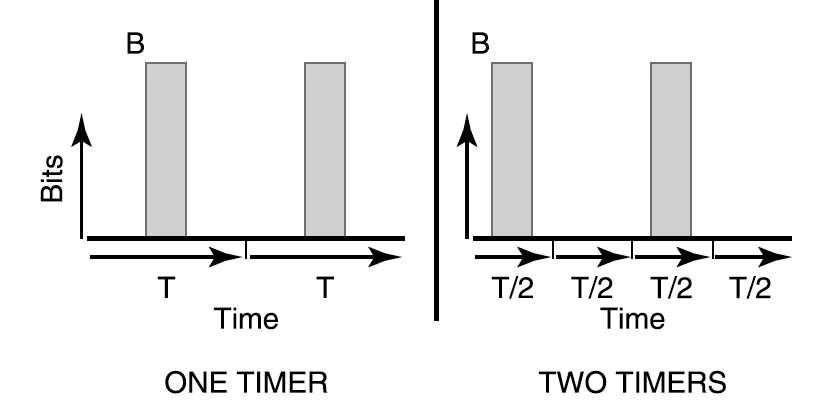
\includegraphics[width=0.8\textwidth]{../assets/ch01/ch01-1_2_网络算法学-020.png}
\end{figure}
图4.20），以便在计时器滴答时检查
是否需要重新传输。然而，当数据包到达X时，TCP还必须快速确定该数据包属于哪个连接，以便更新连
接的状态。每个连接由数据包中携带的连接标识符标识。
依赖于列表来确定数据包的连接在最坏情况下需要搜索整个列表；对于具有大量连接的服务器来说，这
可能很慢。因此，x-kernel实现（Hutchinson和Peterson，1991年）在BSD实现中添加了一个哈希表
（P15），以高效地将数据包中的连接标识符映射到相应的连接状态。哈希表是一个数组，索引由哈希值
指向存储相同哈希值的连接列表。此外，保留了原始的连接列表用于计时器处理，而哈希表用于加速数
据包处理。
                                                                44
然而，对新实现的测量实际上显示了速度变慢！仔细的测量表明，问题在于信息冗余存储，这降低了现
代处理器上数据缓存的效率（参见第2章中的现代处理器模型）。这说明了第3章中的问题Q3，即对系统
的一个部分的明显改进可能会影响系统的其他部分。虽然主内存可能很便宜，但快速内存如数据缓存通
常是有限的。常用的结构如连接列表应尽可能小，以便能够放入数据缓存。
显而易见的解决方案是避免冗余。哈希表用于快速查找。计时器例程还必须定期高效地扫描所有连接。
这导致了以下问题。
问题
能否在保留哈希表的同时消除显式连接列表造成的浪费？可以添加少量额外信息到哈希表。当这样做
时，注意到原始连接列表是双链的，以便在连接终止时轻松删除。然而，这增加了存储并降低了数据缓
存的效率。如何在不使用双链表的情况下使用单链表？
提示：第一部分可以通过将有效的哈希表条目链接在一个列表中来轻松解决。第二部分（避免双链表，
这需要在每个哈希表条目中使用两个指针）稍微困难一些。
连接列表由节点组成，每个节点包含一个连接ID（IP的96位）加上两个指针（假设各32位）以便于删
除。由于哈希表用于快速解复用，如果有效哈希表条目被链接在一起，如\begin{figure}[htbp]
\centering
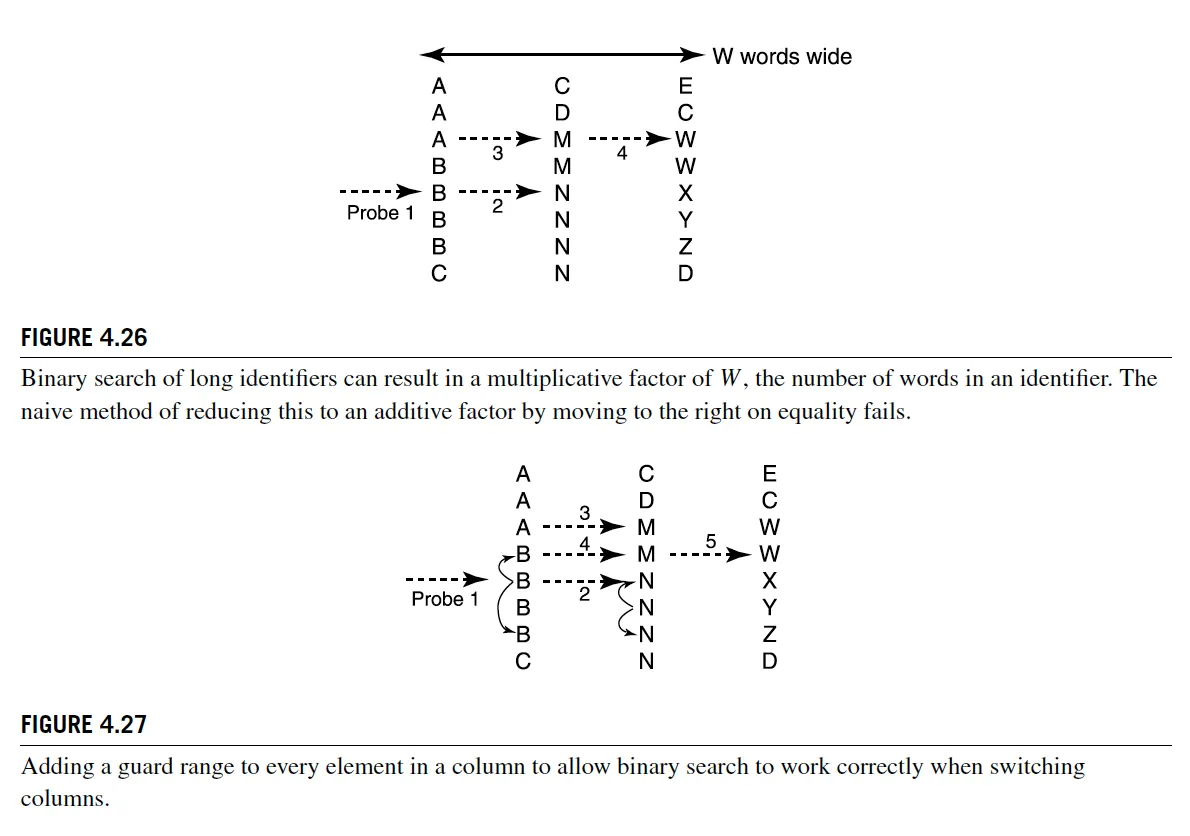
\includegraphics[width=0.8\textwidth]{../assets/ch01/ch01-1_2_网络算法学-021.png}
\end{figure}
图4.21所示，并且保持一个指向
列表头部的指针，则可以移除连接列表。在计时器滴答时，重传例程将定期扫描此列表。完整扫描哈希
表效率较低，因为哈希表可能有许多空位置。
解决方案
双链表仅对高效删除有用。当连接（例如图4.21中的连接C3）终止时，删除例程理想情况下希望找到前
一个有效条目（即图4.21中的包含连接C1的列表），以便将前一个列表链接到下一个列表（即包含C2的
列表）。这需要每个哈希表条目存储一个指向前一个有效条目的指针。
相反，考虑原则P3，该原则询问系统要求是否可以放宽。通常，假设当连接终止时，其存储必须立即回
收。为了回收存储，哈希表条目应放置在空闲列表中，以便可以被另一个连接重用。然而，如果哈希表
比严格需要的稍大，则不必立即重用终止连接的存储。
鉴于这种放宽要求，实现可以延迟删除连接状态。当连接终止时，必须将条目标记为未使用。这需要一
个额外的位状态（如P12），但成本较低。实际删除未使用的哈希表条目E涉及将条目E之前的条目链接
到E之后的条目，并将E返回到空闲列表。然而，这种删除可以在下一次列表遍历时进行，当遍历遇到未
使用的条目时。
练习
●   编写伪代码以添加新连接、终止连接和基于计时器的遍历。

                                                45
● 如何仅使用单链表来实现每个哈希表列表中的连接列表？
● Hugh Hopeful总是对那些他从未彻底思考过的巧妙技巧感兴趣。他建议一种避免在双链表中使用反
  向指针的方法。通常，节点X需要被删除时，删除例程会传递一个句柄来检索X，这通常是一个指向
  节点X的指针。相反，Hugh建议句柄可以是指向链表中X之前节点的指针（除了X是链表头部时句柄
  为空指针）。Hugh声称这允许他的实现在仅使用前向指针的情况下高效地定位X之前和之后的节
  点。提出一个反例来阻止Hugh在编写有缺陷的代码之前继续。
4.12 确认抑制
像TCP这样的传输协议通过要求目的地对每条接收到的数据发送确认（ack）来确保数据被交付给目的
地。这类似于挂号信。数据包和确认都带有编号。确认通常是累积的；对编号为N的数据包的确认隐含地
确认了所有编号小于或等于N的数据包。
累积确认允许接收方灵活地不必为每条接收到的数据包发送确认。相反，确认可以批量处理（P2c）。例
如，在\begin{figure}[htbp]
\centering
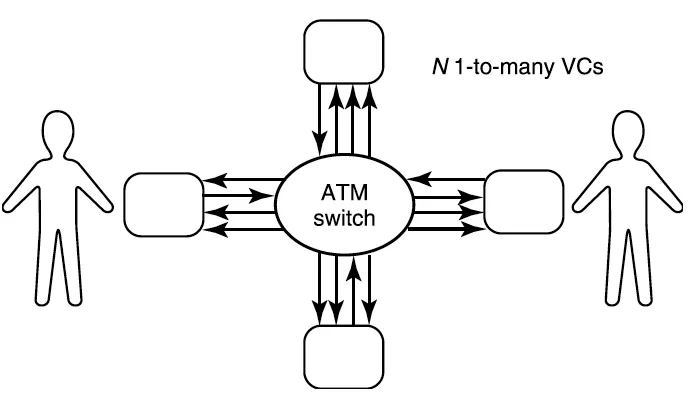
\includegraphics[width=0.8\textwidth]{../assets/ch01/ch01-1_2_网络算法学-022.png}
\end{figure}
图4.22中，文件传输程序正在发送文件块，每个数据包一个块。块1和2分别被确认，但块3和4通
过一个确认块4来确认。
减少确认的数量对发送方和接收方都有好处。尽管确认很小，但它们包含必须由每个路由器和源及目的
地处理的头部。此外，每个接收到的数据包，无论多小，都可能在目的地计算机上引起中断，而中断是
昂贵的。因此，理想情况下，接收方应尽可能批量确认。但是，接收方应该如何制定确认抑制策略以避
免不必要的延迟，同时又能有效地批量确认？
问题
在接收方不是先知的情况下，确认抑制是困难的。例如，在图4.22中，如果块3首先到达并被快速处理，
接收方应该等待块4多久才发送块3的确认？如果块4永远不会到达（因为发送方没有更多数据要发送），
那么抑制块3的确认将导致错误行为。经典的解决方案是设置一个确认抑制计时器；当计时器到期时，发
送累积确认。这限制了确认可以被抑制的时间。
然而，抑制计时器也会导致问题。某些应用程序对延迟敏感。添加确认抑制计时器可能会增加延迟，特
别是在发送方没有更多数据要发送的情况下。如果传输协议可以修改，可以添加什么信息来避免不必要
的延迟，同时又能有效地批量确认？
提示：在像FTP这样的应用程序中，哪个软件模块知道还有更多数据要发送？对于确认抑制，哪个软件模
块理想情况下希望知道还有更多数据要发送？现在考虑使用P9和P10。
解决方案

                                                  46
在像文件传输这样的应用程序中，发送方应用程序知道还有更多数据要发送（例如，将有块4在块3之
后）。发送方应用程序也可能愿意容忍由于确认批量处理而导致的延迟。然而，需要知道此信息的接收
方传输模块。这引出了一个简单的提议。
发送方应用程序向发送方传输层传递一个位（在应用程序-传输接口中），当应用程序有更多数据要发送
时，该位被设置。假设传输协议可以修改以携带一个抑制位。发送方传输层可以使用应用程序传递的信
息来设置每个数据包中的抑制位w；当发送方希望立即确认时，清除该位。关键是发送方传达其意图比接
收方猜测未来更好！
例如，在\begin{figure}[htbp]
\centering
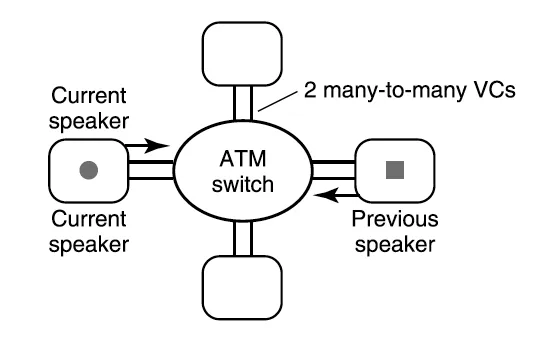
\includegraphics[width=0.8\textwidth]{../assets/ch01/ch01-1_2_网络算法学-023.png}
\end{figure}
图4.23中，发送方传输层被告知发送文件传输应用程序有四个块要发送。因此，发送方传输层
在前三个数据包上设置抑制位，并在第四个数据包上清除该位。接收方根据此信息发送一个确认而不是
四个。另一方面，对延迟敏感的应用程序可以选择不传递有关要发送数据的任何信息。还要注意，抑制
位是一个提示；接收方可以选择忽略此信息并仍然发送确认。尽管这个解决方案看起来很巧妙，但在今
天的TCP中却是一个糟糕的主意。请参阅练习了解更多细节。
练习
● 另一种减少确认的方法是将确认信息附加到从接收方到发送方的数据流中。为了支持这一点，大多
  数传输协议（如TCP）在数据包中有额外的字段来传达反向确认信息。然而，附加确认存在延迟和
  附加确认效率之间的权衡。接收方传输层应该等待多长时间以获取反向数据？另一方面，有许多常
  见应用程序，其中发送方应用程序知道这些信息。如何扩展前面概述的解决方案以支持附加确认以
  及确认批量处理？
● 回想一下第3章中概述的一组用于评估所谓改进的警示问题。例如，问题Q3询问更改是否会影响系
  统的其他部分。为什么激进的确认抑制可能与传输协议的其他方面（如流量控制和拥塞控制
  （Stevens，1994年））相互作用？
4.13 增量读取大型数据库
假设用户连续读取存储在网站上的大型数据库。网页可能会更改，读者只希望获取自上次读取数据库以
来的增量更新（P12a）。因此，在图4.24中，有一个包含广受欢迎食品项目的数据库，全球读者不断阅
读以跟上美食潮流。幸运的是，美食潮流变化缓慢。
因此，一个在下午2点阅读并在下午6点再次阅读的读者只希望获取差异：可口可乐到百事可乐，以及麦
片到 Cheerios。另一方面，如果另一个读者在下午3点阅读并在下午6点阅读，她也只希望获取差异：麦
片到 Cheerios。这导致了以下问题。
问题

                                                  47
找到一种方法，使数据库能够高效地执行此类增量查询。一种解决方案是让数据库记住每个用户上次读
取的内容。然而，要求数据库记住每个用户上次读取的内容是不合理的，因为可能有数百万用户。找到
一种对数据库程序负担较小的解决方案。
提示：如果数据库不存储有关用户上次读取的任何信息，那么用户读取请求必须传递一些信息（P10）关
于同一用户的最后一次读取请求。传递整个上次读取的详细信息将是过度的且低效的。用户上次请求的
最简洁和相关的信息是什么？现在考虑在数据库中添加冗余状态（P12），以便可以使用用户传递的信息
高效地处理增量查询。
解决方案
如前所述，用户读取请求必须传递一些信息（P10）关于同一用户的最后一次读取请求。关于最后一次用
户请求的最简洁和相关的信息是它被执行的时间。如果用户请求传递上次读取的时间T，则数据库需要以
一种高效计算自时间T以来的所有更新的方式来组织。这可以通过存储数据库在所有可能先前时间的副本
来实现。这显然是低效的，可以通过仅存储增量更改（P12a）来避免。这导致了以下算法。
向数据库添加一个更新历史列表，用户读取请求传递上次读取的时间T，因此可以通过扫描更新列表从头
部开始查找自时间T以来的所有更新来处理读取请求。
例如，在图4.25中，更新历史列表的头部是最新的更改（比较图4.24），在下午6点从麦片到
Cheerios，下一个最早的更改是在下午3点从可口可乐到百事可乐。考虑一个读取请求，其上次读取时间
为下午5点。在这种情况下，扫描列表从头部开始，找到下午6点的更新并停止，因为3<5。因此，读取
请求将只返回第一个更新。
练习
● 如果单个条目多次更改，单个条目更改可以在列表中冗余存储，这会消耗空间和时间。可以使用什
  么原则来避免这种冗余？假设数据库只是记录的集合，并且希望每个记录在增量列表中最多出现一
  次。
● 如果记录数量很大或未采用前述技巧，则增量列表的大小将变得非常大。建议一个合理的策略定期
  减少增量列表的大小。
4.14 长标识符的二分搜索
下一代互联网（IPv6）计划使用更大的128位地址以适应更多终端。假设需要对128位地址进行查找，且
算法运行在自然字长为32位的机器上。那么比较两个128位数字需要4次操作（每个字单独比较）。一般
而言，若每个标识符由W个字组成（本例中W=4），朴素的二分搜索需要W·logN次比较，代价高昂。


                                                 48
显然这种方法存在浪费。如果所有标识符的前W-1个字都相同，那么仅需logN次比较即可。问题在于如
何改进二分搜索，使其仅需logN + W次比较。策略是按列处理：从最高有效字开始，在该列进行二分搜
索直至找到匹配项，然后右移到下一列继续搜索。
如图4.26所示（设W=3），假设搜索三字标识符"BMW"（每个字符视为一个字）。首先在左列中间元素
进行比较（图中标为1的箭头）。当搜索字符串的"B"与该位置匹配时，搜索右移到第二列中间位置比
较"M"和"N"。由于N < M，搜索转向第二列的四分之一位置。此时两个"M"匹配，搜索继续右移找
到"W"——但错误地找到了"AMW"而非目标"BMW"。




问题
如何为每列的每个元素添加状态，使得算法能在logN + W次比较内正确工作？
提示：问题根源在于搜索移到第二列四分之一位置时，假设该区域所有元素的左列都以"B"开头。如何通
过添加状态避免这种错误假设？如何修改搜索逻辑来利用这种状态？
解决方案
关键是为每列元素添加守卫范围（guard range）状态。如图4.27所示，对于左列字符（如"B"），添加
指向所有左列同为"B"的元素的指针范围。搜索"BMW"时，首先比较左列"B"（位于"BNX"处）。匹配后
搜索移到第二列，同时记录左列"B"对应的守卫范围（图中第4-7行）。
当发现"M" < "N"时，尝试将搜索范围折半到第三项（"AMW"的"M"）。但该位置低于当前守卫范围下限
（第4行），因此不进行比较直接再次折半到第4项。在此匹配后右移，最终正确找到"BMW"。
                                                     49
通用规则：每个多字条目W1,W2,...,Wn都预计算守卫范围。Wi的范围指向前i个字为W1...Wi的所有条目。
该方案仅需log2N + W次探测，代价是每个字增加两个16位指针（共32位）。由于机器字长通常≥32
位，内存占用最多翻倍。该方案由Butler Lampson提出，核心思想是通过预计算（P2a）换取搜索效
率。


4.15 基于ATM的视频会议系统
图4.28展示了一个ATM交换机连接N个工作站的拓扑。为展示交换机带宽，系统设计者开发了视频会议
应用：任意工作站用户可发起会议，每个参会者屏幕需至少显示当前发言者并播放其语音。多人对话时
还需观察参与者表情。




A videoconferencing system that uses an ATM switch with the ability to support many-to-many
VCs.
问题
最朴素方案需N²个点对点连接，较好方案（图4.28）采用N个一对多VC（虚拟通道），每个工作站视频
流通过独立VC广播给其他参会者。但ATM交换机需静态分配带宽，设单路视频最小带宽Bmin，交换机
总带宽B，则最大参会人数受限于B/Bmin。是否存在更可扩展的方案？
提示：考虑利用交换机硬件支持多对多VC的特性（P4c）。为确保单一发言，可添加硬件（P5）而非复
杂协议。如何通过硬件设计避免多源同时传输？




                                                                                              50
Replacing N one-to-many VCs with two many-to-many VCs through the use of a speech
detector and a simple hardware state machine at each input.
解决方案
如提示所述，设计者选择利用交换机的多对多VC能力，用恒定数量的多对多VC替代N个一对多VC。这使
得固定交换机带宽能够扩展到大量参与者。然而，这一通用思路需要进一步细化：应该使用多少个多对
多VC？如何解决多对多VC可能导致的混乱问题？以下是华盛顿大学Jon Turner提出的具体解决方案细
节。
首先，考虑使用单个多对多VC（命名为C）。解决混乱问题的简单方案是通过协议（例如轮询协议）确
保每次只有一个工作站将其视频输出连接到C。这类协议需要协调，而协调会增加延迟和成本。作为系统
思考者，设计者观察到，至少需要显示当前发言者。因此，设计者在每个工作站的输入端额外添加了语
音检测硬件（P5）。如果检测器在工作站X检测到显著语音活动，则将X的视频输入连接到C；否则，X
的视频输入不与C连接。由于这类硬件成本低廉，扩展性提升的代价非常合理。
接下来，设计者注意到，在典型的双人对话场景中，保留最后一位发言者的视频图像能提供视觉连续
性。因此，他们不再使用单个多对多VC，而是采用两个多对多VC（C和L），分别对应当前发言者和最
后一位发言者，如图4.29所示。




                                                                                    51
